\documentclass[12pt,a4paper]{report}

% ===== PACKAGES =====
\usepackage[utf8]{inputenc}
\usepackage{geometry}
\usepackage{setspace}
\usepackage{titlesec}
\usepackage{fancyhdr}
\usepackage{graphicx}
\usepackage{tocloft}
\usepackage[numbers]{natbib}
\usepackage{amsmath}
\usepackage{amssymb}
\usepackage{booktabs}
\usepackage{longtable}
\usepackage{array}
\usepackage{chngcntr}
\usepackage{microtype}   % smoother line-breaking, fewer overfull-hbox overruns
\usepackage{ragged2e}    % \RaggedRight for cells that must not overflow
\usepackage{tabularx}
% ===== PAGE SETUP =====
\geometry{margin=1in}
\setstretch{1.5}
\setlength{\headheight}{14pt}
\emergencystretch=2em    % lets LaTeX stretch a line slightly instead of spilling into the margin
\sloppy                  % prefer looser spacing over text running past the right margin

% Number tables/figures per chapter (Table 4.1, Figure 3.1, ...)
\counterwithin{table}{chapter}
\counterwithin{figure}{chapter}

% ===== HEADER FOOTER =====
\pagestyle{fancy}
\fancyhf{}
\fancyhead[R]{FPT Institute of Management and Technology}
\fancyfoot[R]{Do Minh Hieu - MSE13172}
\fancyfoot[C]{\thepage}
\renewcommand{\headrulewidth}{0.4pt}
\renewcommand{\footrulewidth}{0.4pt}

% ===== TOC STYLE (đẹp hơn mặc định) =====
\renewcommand{\cftchapfont}{\bfseries}
\renewcommand{\cftchappagefont}{\bfseries}

% Keep the bibliography heading as "References" (report class defaults to "Bibliography")
\renewcommand{\bibname}{References}

% ===== HYPERLINKS (must load after tocloft/natbib/most other packages) =====
% Makes the Table of Contents, List of Tables, List of Figures, and \ref/\cite
% entries actual clickable links that jump to the right page/figure/table/citation,
% and adds PDF bookmarks for navigation.
\usepackage[colorlinks=true, linkcolor=blue, citecolor=blue, urlcolor=blue, bookmarksnumbered=true]{hyperref}

\begin{document}

% ===================== COVER PAGE =====================
\begin{titlepage}
    \centering

    \vspace*{1cm}

    % Logo
    \includegraphics[width=0.45\textwidth]{src-v2/figures/2025-LOGO-FSB.png}

    \vspace{1.5cm}

    {\large \textbf{MASTER'S THESIS}}

    \vspace{1.5cm}

    \rule{0.85\textwidth}{0.5pt}

    \vspace{1cm}

    {\large \textbf{
    SEMANTIC LANE AND TRAFFIC SIGN UNDERSTANDING USING LARGE LANGUAGE MODELS FOR DRIVING DECISION SUPPORT
    }}

    \vspace{0.5cm}

    % NOTE(author): plain pdfLaTeX + inputenc/utf8 cannot render Vietnamese diacritics
    % (o-horn, u-horn, tone marks). Compile with XeLaTeX/LuaLaTeX + fontspec and a
    % Unicode font to enable the line below; left commented out to keep pdfLaTeX builds
    % working out of the box.
    % {\normalsize \textit{(Vietnamese title: Hiểu Làn đường và Biển báo Giao thông
    % theo Ngữ nghĩa sử dụng Mô hình Ngôn ngữ Lớn để Hỗ trợ Ra quyết định Lái xe)}}

    \vspace{1cm}

    \rule{0.85\textwidth}{0.5pt}

    \vspace{2cm}

    \begin{tabular}{rl}
        \textit{Major:} & Software Engineering \\
        \textit{Thesis Supervisor:} & Dr. Doan Nhat Quang \\
        \textit{Author:} & Do Minh Hieu \\
        \textit{Student ID:} & MSE13172 \\
    \end{tabular}

    \vfill

    {\normalsize Hanoi, 2026}

\end{titlepage}
% ===================== FRONT MATTER =====================
% Front matter (Declaration ... List of Abbreviations) uses its own roman-numeral
% page sequence (i, ii, iii, ...), separate from the arabic sequence that Chapter 1
% restarts below -- otherwise both sequences default to arabic and collide/overlap
% in the Table of Contents (e.g. Chapter 1 appearing at a lower page number than
% List of Abbreviations).
\pagenumbering{roman}
\clearpage

\chapter*{Declaration}
\addcontentsline{toc}{chapter}{Declaration}
I hereby declare that this thesis is my own work, carried out under the academic supervision of Dr. Doan Nhat Quang.

The data and experimental results presented in this thesis are truthful, collected and processed using tools and source code that I built myself, and have not been published in any other work. Content referenced from the work of other authors is fully and clearly cited in the References section.

Should any dishonesty or violation of scientific integrity regulations be found, I take full responsibility before the Thesis Committee and the University.

\chapter*{Acknowledgments}
\addcontentsline{toc}{chapter}{Acknowledgments}
To complete this Master's program and this research, beyond my own effort, I have received enormous teaching, guidance, and encouragement from my teachers, my university, my friends, and my family.

First, I would like to express my sincere gratitude to my thesis supervisor, Dr. Doan Nhat Quang. He is the one who inspired and guided me in shaping the idea for this research topic, and who spent a great deal of time instructing me, sharing knowledge, and reviewing and commenting throughout the course of this work. His dedicated guidance not only helped me complete this thesis but will also be valuable groundwork for my professional development going forward.

I sincerely thank the faculty and staff at the FPT Institute of Management and Technology (FSB) for creating a professional, open educational environment in which I could build a solid foundation of specialized knowledge and take part in valuable seminars. I would also like to thank my friends and colleagues, who were always willing to share knowledge, discuss ideas, and accompany me throughout my studies.

Finally, I would like to devote my deepest affection and boundless gratitude to my parents and siblings. My family has always been my firmest anchor, providing peace of mind, trust, and the best possible conditions for me to persevere through difficulties and complete my academic dream.

Despite considerable effort in carrying out and presenting this research, certain limitations remain unavoidable. I sincerely welcome any valuable feedback from the members of the Thesis Committee so that this work can be further improved.

\clearpage
\tableofcontents

\clearpage
\listoftables
\addcontentsline{toc}{chapter}{List of Tables}

\clearpage
\listoffigures
\addcontentsline{toc}{chapter}{List of Figures}

\clearpage
\chapter*{List of Abbreviations}
\addcontentsline{toc}{chapter}{List of Abbreviations}
\begin{longtable}{@{}p{2.2cm}p{4.2cm}p{7.5cm}@{}}
    \toprule
    \textbf{Abbreviation} & \textbf{English} & \textbf{Explanation} \\
    \midrule
    \endhead
    ADAS & Advanced Driver Assistance System & An advanced electronic system that supports driving \\
    XAI & Explainable AI & Explainable AI \\
    LKAS & Lane Keeping Assistance System & A lane-keeping assistance system \\
    VLM & Vision-Language Model & A vision-language model \\
    LLM & Large Language Model & A large language model \\
    MLLM & Multimodal Large Language Model & A multimodal large language model \\
    BEV & Bird's-Eye View & A top-down spatial representation \\
    UFLD-v2 & Ultra Fast Lane Detection v2 & A high-speed lane-detection architecture (version 2) \\
    SCNN & Spatial Convolutional Neural Network & A spatial convolutional neural network \\
    YOLO & You Only Look Once & A family of single-stage object-detection architectures \\
    TSR & Traffic Sign Recognition & Traffic sign recognition \\
    TT100K & Tsinghua-Tencent 100K & A large-scale traffic-sign dataset \\
    MAE & Mean Absolute Error & Mean absolute error \\
    IoU & Intersection over Union & A localization metric \\
    F1 & F1-score & The harmonic mean of Precision and Recall \\
    API & Application Programming Interface & An application programming interface \\
    NIM & NVIDIA Inference Microservices & NVIDIA's model-inference service (the platform used to call the VLM in this thesis) \\
    SSI & Structured Semantic Information & Structured semantic information --- the semantic tuple $S=(\ell,o,c,N)$ and the sign set $D$, derived from raw detection output \\
    JSON & JavaScript Object Notation & The structured data format used to realize SSI \\
    QCVN & Quy chuan Viet Nam (Vietnamese National Technical Regulation) & The Vietnamese national technical-standard system (applies to Vietnamese traffic signs) \\
    \bottomrule
\end{longtable}

% ===================== MAIN CONTENT =====================
\pagenumbering{arabic}
\setcounter{page}{1}

\chapter{Introduction}

\section{Background and Motivation}

Advanced Driver Assistance Systems (ADAS) are on-vehicle electronic systems that use sensors (camera, radar, LiDAR, etc.) to automatically detect traffic situations and support driving behavior --- for example, lane-departure warning, lane-keeping assistance, and automatic emergency braking \cite{nidamanuri2022adas}. This need is tied to the scale of the global road-safety problem: road accidents cause roughly 1.19 million deaths per year \cite{who2023roadsafety}, while lane-departure warning systems have been shown to reduce collision rates by 11\% and related injury rates by 21\% \cite{iihs2017lanedeparture}.

Most current ADAS research focuses on the detection processing step, with lane- and sign-detection modules becoming ever faster and more accurate. However, the output of these modules mainly provides low- or intermediate-level representations such as pixel coordinates, bounding boxes, and class IDs, which do not directly represent the semantic concepts a driver needs to understand a situation (interpretability for humans is a recognized limitation of many AI-based ADAS systems \cite{kuznietsov2024xai}); an intermediate processing step is therefore needed to convert raw detection information into traffic semantics --- lane, offset from center, road shape, and required-compliance signs --- before presenting it to the driver in natural language.

The development of the vision-language model (Vision-Language Model --- VLM) has opened up the possibility of combining visual observation with the generation of driving recommendations in natural language. However, relying entirely on raw pixel data (raw RGB) leaves VLMs facing two major limitations: imprecise spatial localization and a risk of hallucination in complex traffic situations. The principle of supplying additional structured context to increase accuracy and reduce hallucination in a generative model has been validated both in LLMs generally (Retrieval-Augmented Generation \cite{lewis2020rag}) and specifically in driving: DriveVLM \cite{tian2024drivevlm} combines a VLM with structured spatial information to compensate for weak spatial reasoning, while Talk2BEV \cite{choudhary2024talk2bev} shows that placing a VLM on top of a structured map representation clearly improves reasoning quality compared with using the image alone.

\section{Research Gap and Problem Statement}

The principle of supplying structured context noted in Section 1.1 has been validated in LLMs generally and in some specific VLM-based driving systems, but lacks quantitative validation and direct controlled comparison for the task of generating driving recommendations from lane and traffic-sign semantics. The closest existing work --- combining specialized deep learning with VLM/LLM (Section 2.2) --- either stops at integrating structured information to maximize detection accuracy, or focuses on other goals such as spatial reasoning, interaction, or latency optimization; no work has yet quantitatively isolated, through a direct controlled experiment on the same model, the specific contribution of structured semantic information compared with using the raw image alone. This is the specific research gap this thesis aims to fill; a full analysis by group of related work is presented in Section 2.4.

From this gap, the problem this thesis addresses is: to build a pipeline that converts the raw output of traffic-infrastructure detection models into structured semantic information, and to quantitatively verify, through a controlled experiment, whether this information improves the quality of VLM-generated driving recommendations compared with using the raw image alone. Because the full space of traffic semantics covers many other factors (surrounding vehicles, dynamic obstacles, etc.), the problem is narrowed to the two most fundamental, fixed infrastructure components --- lanes and traffic signs (the specific scope is given in Section 1.4).

\section{Objectives and Research Questions}

The central hypothesis of this study, stated in a testable form: the average recommendation-quality score rated by the LLM-as-a-judge in the mode with SSI (Structured Semantic Information --- a structured data representation comprising the ego lane, lane count, offset from center, road shape, and signs) will be statistically significantly higher than in the mode using only the raw input image. From this hypothesis, the thesis focuses on answering the core research question:

\begin{quote}
\textit{``To what extent does integrating SSI improve the quality, accuracy, and groundedness of VLM-generated driving recommendations compared with relying solely on raw image data?''}
\end{quote}

Building on this question and the problem stated in Section 1.2, the overall objective of this thesis is to build and quantitatively verify a pipeline that converts raw traffic-infrastructure detection data (lanes, signs) into SSI, serving as supplementary context for a Multimodal Language Model (VLM) in the task of generating natural-language driving recommendations. Three specific objectives, each addressing a distinct gap in that processing chain:

\begin{enumerate}
    \item \textbf{Develop a semantic-representation module}: Design and implement a module that converts the raw output of specialized lane- and traffic-sign-detection models into SSI, including information such as lane count, ego lane, offset from center, neighbor lanes, road shape, and sign information.
    \item \textbf{Design a mechanism for supplying SSI to the VLM}: Build and standardize a prompt to supply SSI together with the input image to the VLM, guiding the model to exploit structured semantic information when analyzing a situation and generating a driving recommendation. The manner of supplying this information is controlled consistently to ensure fairness across the comparative experiments.
    \item \textbf{Quantify the impact of SSI and verify the reliability of the evaluation}: Use LLM-as-a-Judge to evaluate recommendation quality across different input modes, while verifying the reliability of the evaluation itself through comparison with human evaluation and consistency across multiple judges.
\end{enumerate}

\section{Research Scope}

Because the full space of traffic semantics covers many factors (road infrastructure, surrounding vehicles, dynamic obstacles, etc.), to ensure feasibility this thesis narrows its scope to the two most fundamental, fixed infrastructure components --- lanes and traffic signs --- which directly determine spatial positioning and the mandatory rules applicable to a vehicle.

For data, this thesis performs quantitative verification on two internationally recognized public standard datasets --- CULane \cite{pan2018culane} for the lane task, TT100K \cite{zhu2016tt100k} for the traffic-sign task --- to ensure reproducibility and objective comparison with related work, and additionally supplements this with a self-collected dataset, independent of UFLD-v2's training data, to verify the ability to generalize beyond the training distribution.

\section{Main Contributions}

The contributions of this thesis center on building and verifying a \textbf{multi-model framework} that combines structured semantic information from lane- and sign-detection models with a VLM for the task of natural-language driving decision support. The focus of this research is not merely building a multi-model pipeline, but quantifying the added value of structured semantic information to VLM recommendation quality through a controlled experimental design. The specific contributions are:

\begin{enumerate}
    \item \textbf{Technical contribution --- A structured semantic-representation module for lane and traffic-sign information:} Building a pipeline that converts the output of specialized detection models into SSI, comprising semantic attributes such as lane count, ego lane, offset from center, neighbor lanes, road shape, and sign information. SSI's accuracy is verified against ground truth on both benchmark data and self-collected data, thereby assessing how well-suited this representation is as supplementary input for a VLM.
    \item \textbf{Methodological contribution --- A controlled experimental design to evaluate the added value of SSI:} Building a comparison framework across three input modes --- image-only, SSI-only, and image combined with SSI --- on the same VLM, the same image set, and the same evaluation criteria. This design enables the incremental contribution of SSI to recommendation quality to be assessed separately, while limiting the influence of unrelated experimental factors.
    \item \textbf{Experimental contribution --- Quantitative evidence of SSI's impact and the reliability of the evaluation:} Conducting a controlled experiment on the evaluation dataset and analyzing the results with multiple independent judges. The reliability of LLM-as-a-Judge is verified through consistency across judges and comparison with human evaluation, thereby providing an experimental basis for answering the research question on the value of SSI for VLM-based driving decision support.
\end{enumerate}

\section{Thesis Structure}

The full thesis is organized into 5 main chapters, presented in the following logical order:

\textbf{Chapter 1: Introduction.} Presents an overview of the research background, the motivation for the topic, the research gap and problem, the objectives and research questions, the research scope, and the main contributions of the thesis.

\textbf{Chapter 2: Literature Review and Related Work.} Presents the theoretical background and an overview of related work across three main content groups --- lane and traffic-sign detection, the application of Vision-Language Models (VLMs) to traffic problems, and the LLM-as-a-Judge evaluation methodology --- thereby clearly identifying the knowledge gap this thesis aims to address.

\textbf{Chapter 3: Methodology.} Describes in detail the overall system architecture, the data collection and processing pipeline, the infrastructure semantic-extraction algorithms (lanes and signs), the design of the structured semantic representation, prompt engineering, and the evaluation methodology framework.

\textbf{Chapter 4: Results and Discussion.} Presents in detail the experimental configuration, the quantitative results of each component module, the central experimental result on SSI's impact on the VLM, verification of LLM-as-a-Judge reliability, in-depth analyses clarifying the actual mechanism behind that information's contribution, together with an objective discussion of the remaining limitations.

\textbf{Chapter 5: Conclusion.} Summarizes the main contributions, consolidates the answers to the research questions, and proposes directions for future research.

\textbf{Summary of Chapter 1.} Chapter 1 has analyzed the research background and motivation, and identified the specific research gap and problem this thesis addresses. On that basis, this chapter has established the objectives and research questions, the research scope, and the core contributions of the thesis. The following Chapter 2 presents an overview of related work to further clarify the theoretical foundation and scientific basis for the proposed methodology.

\chapter{Literature Review and Related Work}

Advanced Driver Assistance Systems (ADAS) are now an almost standard feature in commercial vehicles, with widely available features such as lane-departure warning, lane-keeping assistance, and traffic-sign recognition; they are also the necessary perceptual foundation for progressing toward higher levels of automation. Nidamanuri et al. \cite{nidamanuri2022adas} survey the evolution of ADAS technology across automation levels, showing a trend of shifting from single-sensor systems toward multi-sensor systems combined with deep learning to increase reliability under diverse real-world conditions. Alongside the requirement for accuracy, the explainability of AI-made decisions is increasingly regarded as an important condition for ADAS to be deployed and accepted at scale, particularly in edge cases: Kuznietsov et al. \cite{kuznietsov2024xai} conduct the first systematic review of Explainable AI (XAI) for safe autonomous driving, identifying five main contributions of XAI --- interpretable design, interpretable surrogate models, interpretable monitoring, auxiliary explanation, and interpretable verification. Tselentis and Papadimitriou \cite{tselentis2023driverprofile} add a human-factors dimension that purely sensor-based ADAS systems tend to underexploit: recognizing driver profile and driving pattern as an input signal for traffic-safety assessment. These three research directions --- sensor technology, explainability, and human factors --- together sketch the broader context this thesis contributes to: building a decision-support layer that is both accurate and interpretable in natural language.

\section{Lane and Traffic Sign Detection}

\subsection{Lane Detection}

Lane detection is the task of locating lane markings/boundaries in an image, providing a direct basis for ADAS lane-departure warning and lane-keeping assistance features. Over roughly the past decade, the approach to this task has shifted markedly from traditional geometric methods (edge detection, Hough transform, polynomial fitting) toward deep-learning architectures, owing to their better handling of complex real-world conditions such as shadows, faded markings, or changing lighting. Within the deep-learning family, three main design families have emerged: (a) semantic segmentation --- treating each pixel as belonging to a lane or not; (b) ordinal classification over a row/column grid --- predicting lane position at discrete image rows rather than regressing coordinates directly; and (c) anchor-based mechanisms --- proposing a set of candidate lines/regions in advance and then refining them. These three families trade off geometric accuracy against inference speed in different ways.

For evaluation, standard benchmarks for this task typically report metrics at the point-wise localization level, typically F1 at an IoU threshold between the predicted lane and ground truth. This is a fundamentally different kind of metric from higher-level semantic quantities --- for example lane count, ego lane, road shape --- which require a separate post-processing step to derive from raw point-wise detection output; these two kinds of metrics cannot be directly compared.

Ultra-Fast-Lane-Detection-v2 (UFLD-v2) \cite{qin2022ufldv2} is a high-speed lane-detection architecture representative of the hybrid anchor-driven ordinal classification family. This architecture achieves an inference speed above 300 frames per second in its lightweight version, while retaining competitive accuracy --- F1 = 76.0\% on the CULane test set with a ResNet-34 backbone, exactly the pretrained variant (\texttt{culane\_res34.pth}) this thesis uses as-is in Section 3.1. CULane \cite{pan2018culane} is the standard benchmark for this task (88.9 thousand training images, 9.7 thousand validation images, 34.7 thousand test images), with data mainly characterized by diverse urban road situations: intersections, high traffic density, and varying lighting conditions.

\begin{figure}[h!]
    \centering
    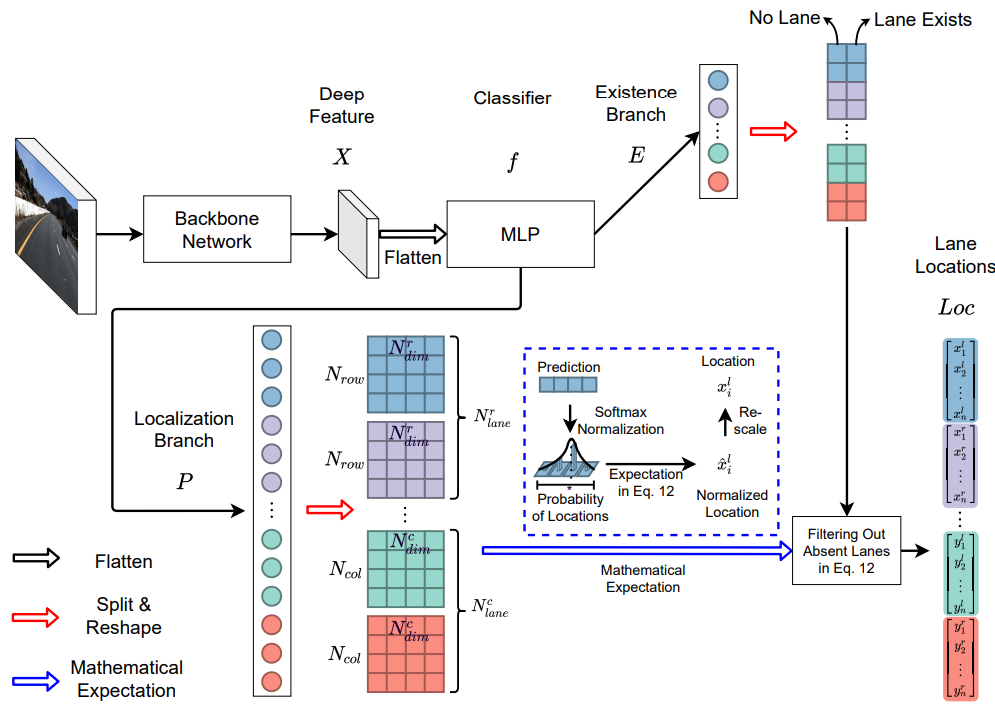
\includegraphics[width=0.85\textwidth]{src-v2/figures/ufldv2.png}
    \caption[Overall architecture of UFLD-v2]{Overall architecture of UFLD-v2 (source: \cite{qin2022ufldv2}). A Backbone Network extracts deep features $X$ from the input image, fed through a classifier (MLP) $f$ that produces two parallel prediction branches: the Existence Branch $E$ predicts whether each boundary actually exists (No Lane/Lane Exists); the Localization Branch $P$ predicts position over a row/column grid ($N_{row}$/$N_{col}$ cells), then applies mathematical expectation over the position probability distribution --- rather than simply taking the class with the highest probability --- to derive a more precise continuous coordinate (Loc). Boundaries predicted as ``No Lane'' by the Existence Branch are removed from the final output (Filtering Out Absent Lanes). This is exactly the ``hybrid anchor-driven ordinal classification'' mechanism noted above: combining existence classification with ordinal classification over a row/column grid, instead of directly regressing coordinates.}
    \label{fig:ufldv2}
\end{figure}

Representing the anchor family, LaneATT \cite{tabelini2021laneatt} and CLRNet \cite{zheng2022clrnet} extend in two different directions --- line-anchors combined with attention to enable a lightweight backbone, and cross-layer refinement with a Line IoU loss that directly measures geometric fit --- both achieving high accuracy on CULane at the time of publication. The survey by He et al. \cite{he2024monocularsurvey} systematizes four main design axes of the field (task modeling, lane parameterization, global context for occluded lanes, and perspective removal for the 3D problem); two earlier surveys \cite{zhang2021survey,zakaria2023slr} likewise note the shift from traditional geometric models toward deep learning. A common thread across this group: the metrics being optimized (F1/IoU, inference speed) are measured at the point-wise detection level, a different kind of quantity from the decision-level semantics --- lane count, ego lane, road shape --- that this thesis targets (Section 2.1.1).

Beyond improving detection algorithms, evaluating the real-world deployment quality of Lane Keeping Assistance Systems (LKAS) is itself a separate line of research. Wei et al. \cite{wei2024lkas} survey existing LKAS evaluation methods --- from the group of objective metrics (lane deviation, reaction time) to the group of methods that incorporate the driver's subjective perception --- and note that the latter group remains less standardized.

\subsection{Traffic Sign Detection}

Traffic Sign Recognition (TSR) is the task of localizing and classifying traffic signs in an image, directly serving driver-assistance/compliance-reminder features. Architecturally, two common approaches are two-stage detectors (proposing candidate regions and then classifying them, e.g., Mask R-CNN) and single-stage detectors (predicting location and class simultaneously in a single inference pass, e.g., the YOLO family, trading accuracy for speed). Task difficulty depends strongly on the number of target classes (a few dozen classes for typical driving applications versus hundreds of classes for large-scale sign inventories) and object size in the image --- signs that are far away or captured at an angle often occupy only a very small region, a common challenge for single-stage architectures. For evaluation, two tasks of different difficulty must be distinguished: classification on an already-cropped region, typically reported by Accuracy; and detection from scratch (detection) over the full frame with no prior location hint, typically reported by Precision/Recall --- the latter task is considerably harder because it combines both localization error and classification error.

YOLOv8 (Ultralytics) inherits the YOLO family of architectures --- single-stage object detection that predicts location and class simultaneously in one inference pass, rather than separating out a candidate-region-proposal step as two-stage detectors do \cite{redmon2016yolo} --- now widely used for the TSR task owing to its good balance of speed and accuracy, suitable for real-time applications. TT100K (Tsinghua-Tencent 100K) \cite{zhu2016tt100k} is a large-scale benchmark for traffic-sign detection and classification in China, comprising roughly 100,000 images and 30,000 labeled sign instances, with a detailed sign-encoding scheme by category: prohibition signs (``p''), mandatory signs (``i''), warning signs (``w''), and speed-limit signs (``pl''/``il'').

Before YOLO, the two-stage approach had already proven effective at a much larger scale --- Tabernik and Sko{\v c}aj \cite{tabernik2020largescale} use Mask R-CNN for hundreds of sign types --- showing that TSR difficulty depends strongly on the number of target classes, not just on the architecture. Recent work integrates attention/transformer mechanisms into YOLOv8 to improve small-object detection: Logeswaran et al. \cite{logeswaran2024pedestrian} confirm the feasibility of simultaneously detecting pedestrians and traffic signs; Ji et al. \cite{ji2024improvedyolov8} add BoTNet, ODConv, and LSKA to YOLOv8n, improving accuracy on small objects on TT100K. This group of work optimizes single-sign detection/classification accuracy but has not linked detection results to reasoning about the corresponding traffic rules --- a processing step this thesis performs in the semantic-analysis module (Section 3.3).

\section{Vision-Language Models (VLMs) for Traffic Applications}

A Vision-Language Model (VLM) extends a text-only LLM to accept both an image and text as input simultaneously, typically following an architecture with three components: a visual encoder that extracts features from the image, a projection layer that maps visual features into the LLM's embedding space, and the LLM itself, which generates text conditioned on the combined multimodal embedding sequence. There are two ways to adapt a VLM to a specific task: fine-tuning all or part of the model on specialized data to optimize performance for that exact task, or using a pretrained general-purpose VLM as-is (training-free), exploited purely through prompt engineering without updating model parameters. The second approach has considerably lower deployment cost but depends more heavily on the quality of the context and prompt supplied to the model.

Work applying VLM/LLM to traffic can be grouped by the model's role in the pipeline, ranging from end-to-end systems to an added interaction/reasoning layer and hybrid architectures, summarized in Table 2.1, before a detailed analysis of each group.

\begin{table}[htbp]
    \centering
    \footnotesize
    \caption{Summary of related work on LLM/VLM for driving.}
    \label{tab:2.1}
    \begin{tabularx}{\linewidth}{@{}p{2.6cm}p{2.4cm}Xp{3.6cm}@{}}
        \toprule
        \textbf{Group} & \textbf{Work} & \textbf{Main technical characteristics} & \textbf{Notable published results} \\
        \midrule
        Large-scale end-to-end & DriveGPT4 \cite{xu2024drivegpt4} & Generates natural-language explanations alongside control signals, trained end-to-end & --- \\
         & DriveLM \cite{sima2024drivelm} & Frames driving as Graph Visual Question Answering & --- \\
         & LMDrive \cite{shao2024lmdrive} & Closed-loop end-to-end driving with an LLM & --- \\
        Added interaction/ reasoning layer & Drive as You Speak \cite{cui2024driveasyouspeak} & LLM tool-use, reasoning-acting, personalized interaction & --- \\
         & DriveVLM \cite{tian2024drivevlm} & Hybrid DriveVLM-Dual architecture: VLM + traditional pipeline for spatial reasoning & Verified on nuScenes + real-world deployment \\
         & Confidence-aware lightweight LM \cite{yao2026confidenceaware} & Distilled from a multi-agent system, confidence-aware & SOTA on the nuPlan benchmark, low latency \\
         & Talk2BEV \cite{choudhary2024talk2bev} & VLM on a bird's-eye-view representation, no task-specific training & Talk2BEV-Bench, $>$20{,}000 questions on nuScenes \\
        Hybrid deep learning + MLLM & SafeRoute \cite{shaw2025saferoute} / Advancing-AV-Intelligence \cite{sah2025advancing} & Multimodal Adapter fusing CNN features with EVA-CLIP embeddings & ResNet-50 99.8\% / YOLOv8 98.0\% / RT-DETR 96.6\% (signs); Question Overall Accuracy 82.83\% (lanes) \\
         & DSC-LLM \cite{kim2025dscllm} & Behavioral features (LSTM/transformer) + image context, trajectory prediction & --- \\
        \bottomrule
    \end{tabularx}
\end{table}

\textbf{Predecessors before the LLM era.} Hong et al. \cite{hong2019rules} laid the groundwork for the idea of encoding high-level traffic-situation semantics into a structured representation (a spatial-grid form) for a deep-learning model to reason about driving behavior. This work uses a purely convolutional network; its only limitation is that it does not generate natural-language explanations --- something later large language models would go on to solve.

\textbf{VLMs for traffic semantic understanding, not directly tied to control decisions.} Alongside VLM/LLM systems tied to the control loop or to generating behavioral recommendations (Table 2.1), another research branch uses VLMs purely for describing and understanding traffic-scene semantics, not necessarily aiming to generate behavioral recommendations. Rivera et al. \cite{rivera2025scenario} use general-purpose VLMs (GPT-4, LLaVA) to automatically classify and semantically annotate urban traffic scenes on BDD100K without retraining on each new label set --- direct evidence that general-purpose VLMs can understand traffic context in a training-free setting. Fan et al. \cite{fan2024mllmsul} (MLLM-SUL) go a step further: combining a dual-branch visual encoder with a fine-tuned LLM to simultaneously generate a semantic scene description and localize risk regions in the image --- a fine-tuned, specialized-MLLM approach, closer to the hybrid group in Table 2.1. Both works show that VLMs' ability to understand traffic semantics is being exploited in multiple directions --- from automating data labeling to risk localization --- but mostly focus on the scene's overall semantics (situation type, objects, risk level), without going deep into structured lane and traffic-sign semantics.

\textbf{Large-scale end-to-end VLM/LLM driving systems.} With the emergence of multimodal large language models, an active research direction has formed to integrate language-reasoning capability directly into the end-to-end driving pipeline --- represented by DriveGPT4 \cite{xu2024drivegpt4}, DriveLM \cite{sima2024drivelm}, and LMDrive \cite{shao2024lmdrive} (Table 2.1). These systems achieve interpretability deeply integrated right into the control loop, at the cost of requiring training or fine-tuning on large-scale driving datasets (nuScenes, CARLA, etc.) along with significant compute and data infrastructure.

\textbf{LLM/VLM systems as an added interaction/reasoning processing step.} A recent group of work uses LLM/VLM as an added reasoning or interaction processing step attached to an existing driving pipeline --- Drive as You Speak \cite{cui2024driveasyouspeak}, DriveVLM \cite{tian2024drivevlm}, the confidence-aware lightweight language model \cite{yao2026confidenceaware}, and Talk2BEV \cite{choudhary2024talk2bev} (Table 2.1). Notably, DriveVLM \cite{tian2024drivevlm} explicitly acknowledges a limitation of pure VLMs in spatial reasoning and therefore combines them with a traditional pipeline to compensate. Yao et al. \cite{yao2026confidenceaware} address the reasoning-cost problem --- an important constraint for real-time deployment --- by distilling a confidence-aware lightweight language model from a multi-agent system. These four works target different goals: improving interaction and personalization \cite{cui2024driveasyouspeak}, extending spatial reasoning in complex situations \cite{tian2024drivevlm}, optimizing inference cost/latency \cite{yao2026confidenceaware}, or extending the representation space to BEV \cite{choudhary2024talk2bev}.

\textbf{Hybrid deep learning + MLLM systems.} SafeRoute \cite{shaw2025saferoute} and its predecessor work ``Advancing Autonomous Vehicle Intelligence'' \cite{sah2025advancing} --- from the same group of authors --- build a unified pipeline fusing CNN features with language embeddings at the representation level (Table 2.1), achieving high accuracy in both sign recognition and lane understanding --- showing that fusing information at the embedding level delivers strong performance given sufficient data and resources to fine-tune the MLLM. Similarly, DSC-LLM \cite{kim2025dscllm} combines behavioral features with traffic context extracted from images to predict trajectories along with LLM-explained risk reasoning.

\section{LLM-as-a-Judge Evaluation Methodology}

Evaluating the quality of natural-language output is a task that is hard to quantify with traditional hard metrics (accuracy, F1, etc.) because there is no ``single correct answer''. The LLM-as-a-judge method --- using a strong LLM as an automated ``judge'' that scores against a given rubric --- addresses this by replacing human evaluation with a model strong enough to capture linguistic nuance, at the cost of facing inherent biases already documented in the literature, notably in the MT-Bench study itself \cite{zheng2023mtbench}: length bias (longer answers tend to be scored higher even when no more accurate), style bias (a confident, well-structured writing style is rated more highly than the actual factual content), and self-preference bias among models from the same family. These biases need to be verified separately for each specific application task; an LLM-as-a-judge cannot be assumed reliable merely because it has been validated on a different benchmark.

The LLM-as-a-judge methodology has been widely applied in recent LLM evaluation benchmarks, notably MT-Bench and Chatbot Arena \cite{zheng2023mtbench}, as well as AlpacaEval. On MT-Bench, GPT-4 acting as judge reaches 85\% agreement with human experts (on non-tied comparison pairs), a level approaching human-to-human agreement (81\%) --- suggesting that LLM-as-a-judge can approach human-level reliability under suitable conditions. A recent survey \cite{ferrag2025review} systematizes LLM/agent evaluation benchmarks and frameworks published between 2019 and 2025, showing this remains a field still taking shape, without a unified methodology.

Because manually scoring the entire dataset to verify an evaluation tool is often infeasible, several recent studies propose small-scale, purposive human-sampling frameworks: Kim \cite{kim2026augmenting} proposes a two-stage sampling framework --- the LLM scores the entire dataset, and humans score only a purposively selected subsample at the points where the LLM's predictions are least reliable --- and emphasizes that the literature currently lacks formal guidance on how much human oversight is sufficient when validating a benchmark. Saha et al. \cite{saha2026budget} propose allocating queries adaptively by variance rather than uniformly, to reduce estimation error under a fixed compute budget. Pan et al. \cite{pan2024human} interview eight experts and emphasize the need for support in building evaluation criteria that match real users' expectations.

The quality of the evaluation data itself --- not only the quality of the evaluation tool --- is also a concern raised in recent literature. Emami et al. \cite{emami2024humanintheloop} review the role of human-in-the-loop in training/validation for safe and ethical autonomous vehicles, emphasizing that data labeling remains the main bottleneck. Fern{\'a}ndez Llorca et al. \cite{fernandezllorca2024bias} assess bias in popular vision datasets for autonomous vehicles, finding very low diversity across many pedestrian demographic attributes --- a reminder that even standard datasets may carry unverified latent biases.

\section{Summary of the Research Gap}

The literature review shows that structured information has been exploited in many VLM/LLM traffic systems in various forms, such as spatial representations, BEV, control signals, or embedding-level features. However, these studies mainly target goals such as spatial reasoning, trajectory prediction, interaction, or system performance optimization. Meanwhile, there is not yet sufficient direct experimental evidence for the question of whether a structured semantic representation, built from the output of lane- and traffic-sign-detection models, creates added value for a VLM when generating driving recommendations. Specifically, the research gap this thesis addresses lies in three closely related aspects:

\textbf{Gap in intermediate semantic representation:} Existing work uses many different forms of structured representation, but none has focused on a lightweight lane- and sign-level semantic representation, built from the output of specialized perception models and used directly as context for a general-purpose, non-fine-tuned VLM.

\textbf{Gap in verifying the impact of semantic information:} Existing studies have not focused on controlled verification of the value of this semantic information itself for recommendation quality, isolated from the VLM's own ability to perceive from the image.

\textbf{Gap in reliable evaluation of language output:} Because the recommendation output is natural language and hard to evaluate with hard metrics, a sufficiently reliable evaluation method is needed to compare input conditions; verifying LLM-as-a-Judge by comparison with humans and across multiple judges therefore becomes a methodological requirement of this study.

From the above gaps, this thesis focuses on the core question: does SSI, built from lane and traffic-sign information, create a significant added value for a VLM in the driving decision-support task, and if so, to what extent does the improvement manifest across different evaluation criteria?

To answer this question, this study builds a pipeline consisting of specialized detection models, a module that converts their output into SSI, a mechanism for supplying SSI to the VLM via prompt, and an evaluation framework with verified reliability. The value of SSI is verified through a controlled experiment across three input modes: image-only, SSI-only, and image combined with SSI, on the same VLM and the same evaluation dataset.

\textbf{Chapter summary.} This chapter has presented the theoretical foundation and an overview of related work for the thesis's three components --- lane and traffic-sign detection, multimodal large language models, and the LLM-as-a-judge evaluation methodology --- and identified three specific research gaps, corresponding directly to the three research objectives stated in Section 1.3, which this thesis contributes to filling. The following Chapter 3 presents in detail the methodology built to address those gaps, starting from the overall system architecture.

\chapter{Methodology}

Before presenting each component in detail, this introductory section formally states the lane-semantics problem this thesis addresses, establishing unified notation for the entire chapter.

\textbf{Input.} The processing unit for the whole pipeline is a single dashcam image $I$ --- a still frame taken from a trip video or captured directly, processed independently under the single-frame assumption stated above. $I$ is a 3-channel color (RGB) image; its size $W \times H$ (pixels) varies by data source (1640$\times$590 for CULane, 1280$\times$720 for the real-life set).

The UFLD-v2 lane-detection model takes $I$ as input and returns a set of boundaries $B = \{b_1, b_2, \ldots, b_n\}$, where each boundary $b_i$ is a list of pixel points $\{(x, y)\}$ along an observed lane marking --- this is raw, pixel-level output that does not yet carry decision-level semantics. The \textbf{task} of the lane-semantic-extraction module (Section 3.3.1) is to map this raw set of boundaries $B$ into a decision-level semantic tuple $S = (\ell, o, c, N)$, where:

\begin{itemize}
    \item $\ell$ (ego lane) --- the pair of boundaries $(b_i, b_{i+1}) \subset B$ that defines the lane the vehicle is currently in, with an accompanying confidence value;
    \item $o$ (vehicle offset) --- the offset $\Delta x$ between the center of the ego lane and the center of the image, expressed both in pixels and as a percentage of lane width;
    \item $c$ (road shape) --- the classification of the overall road shape (straight/gentle curve/sharp curve --- \texttt{straight}/\texttt{gentle}/\texttt{sharp} in the output), together with curve direction;
    \item $N$ --- the number of neighbor lanes to the left/right of the ego lane.
\end{itemize}

In parallel, the YOLOv8n sign-detection model takes $I$ as input and returns a set $D = \{(cls_j, box_j)\}$ of class labels and bounding-box coordinates for each detected traffic sign.

\textbf{On representation format.} The semantic tuple $S$ and the set $D$ are themselves abstract data structures --- a set of values and labels --- not tied to any specific serialization format. The relationship among $S$, $D$, and SSI is stated explicitly through a transformation $\Phi$:

\[
SSI = \Phi(S, D)
\]

where $\Phi$ is the normalization and serialization of $S$/$D$ into a single structured character string; JSON is the specific format chosen to realize $\Phi$ --- this is the concrete instantiation of SSI, both embedded in the prompt in the SSI-only and combined modes, and used as the basis for automated comparison against ground truth throughout Chapter 4 (the semantic content of each information field is presented in Section 3.3.3).

The semantic tuple $S$ and the set $D$, once normalized into a single JSON representation (SSI, Section 3.3.3), serve as input to the reasoning processing step: a multimodal large language model $M$ receives the image $I$ and/or SSI, and generates a driving recommendation $R$ as structured, three-part natural-language text (Section 3.4). The core research question (Section 1.3) is precisely the quantitative comparison of $R$'s quality when $M$ receives, in turn, $(I)$, $(S)$, or $(I, S)$ as input --- the thesis calls these three ways of supplying input the \textbf{image-only mode} $(I)$, the \textbf{SSI-only mode} $(S)$, and the \textbf{combined mode} $(I,S)$. In the source code and API call configuration, these three modes are identified respectively as \texttt{image\_only}, \texttt{json\_only}, and \texttt{image\_json} (or \texttt{image+json}); from here on, the entire thesis --- including the column names in the data tables in Chapter 4 --- uses these descriptive names (image-only, SSI-only, combined) rather than these technical identifiers.

\textbf{System assumptions.} The following six assumptions govern the entire pipeline and need to be stated explicitly once here, rather than appearing scattered throughout the technical description:

\begin{enumerate}
    \item \textit{Independent, single-frame processing} --- no information from preceding/following frames is used, and there is no tracking step between consecutive frames.
    \item \textit{No use of temporal information} --- every image is reasoned about independently of any observation history, even when the source is a video.
    \item \textit{The camera is assumed to be mounted near the horizontal center of the vehicle} (Section 3.3.1) --- every computation of the offset from center $o$ and the ego lane $\ell$ relies on this assumption; real-world mounting deviation is handled through the calibration parameter $o_c$.
    \item \textit{No explicit depth estimation} --- the physical distance to a sign or another vehicle is neither measured nor estimated anywhere in the pipeline.
    \item \textit{Inferred semantics depend entirely on the output of the detection layer} --- if UFLD-v2/YOLOv8n misses or misdetects something, the semantic-analysis module has no compensating mechanism; errors at the detection layer propagate directly into SSI.
    \item \textit{Reasoning about signs and rules is limited strictly to signs the detector has actually detected} --- the system does not infer the existence of signs that are not present in YOLOv8n's output.
\end{enumerate}

Sections 3.1--3.6 below present each pipeline component in detail, in processing order: the overall architecture (Section 3.1), the data and preprocessing (Section 3.2), the SSI-extraction module --- the algorithm that derives $S$ from $B$, sign semantics from $D$, and the complete SSI structure (Section 3.3) --- the prompt-engineering design that generates $R$ (Section 3.4), the controlled experiment design and the framework for evaluating $R$ --- including the choice of model $M$, the input modes, the evaluation criteria, and statistical testing (Section 3.5) --- and a concrete end-to-end illustrative example (Section 3.6).

\section{Overall System Architecture}

The pipeline of this thesis comprises four sequential processing stages, illustrated in Figure~\ref{fig:pipeline}: two deep-learning-based processing steps (detection, reasoning), connected through a purely algorithmic semantic-processing module --- containing no learned parameters --- and closed off by an evaluation processing step. The English name in parentheses at each stage is the standard term used consistently throughout the thesis.

\begin{figure}[h!]
    \centering
    \includegraphics[width=0.85\textwidth]{src-v2/figures/hinh\_3\_1\_kien\_truc.png}
    \caption[Overall architecture of the four-stage pipeline]{Overall architecture of the four-stage pipeline. The dashed border of module 2 visually marks a distinction: this is an algorithmic/rule-based module, not a deep-learning-based processing step like the other three stages (legend at the bottom of the figure).}
    \label{fig:pipeline}
\end{figure}

Calling stage 2 a ``module'' --- rather than using the common name ``processing step'' as for the other three stages --- is deliberate: unlike the other three stages --- detection (UFLD-v2, YOLOv8n), reasoning (VLM), evaluation (LLM-as-a-judge) --- which are all trained models, the semantic-analysis module is a self-designed sequence of rules and geometric formulas (Section 3.3) with no learned parameters --- the name ``module'' clearly marks this distinction.

\textbf{Models used in the detection processing step.} The first stage comprises two independent specialized detection models, run in parallel on the same input image $I$:

\begin{itemize}
    \item \textit{Lane detection}: UFLD-v2, ResNet-34 backbone, used as-is, pretrained on CULane (\texttt{culane\_res34.pth}), with no further fine-tuning.
    \item \textit{Sign detection}: YOLOv8n (the smallest variant in the YOLOv8 family, about 3.2 million parameters), self-fine-tuned on a 51-class common subset of TT100K, initialized from the original YOLOv8n checkpoint (pretrained on COCO). Training configuration:
    \begin{itemize}
        \item Input image resolution: 640$\times$640; automatic batch size (\texttt{batch=-1}).
        \item SGD optimizer, initial learning rate \texttt{lr0=0.01}, momentum \texttt{0.937}, weight decay \texttt{0.0005}, 3-epoch warm-up.
        \item Up to 100 epochs, with early stopping \texttt{patience=30} (stop if no improvement after 30 consecutive epochs).
    \end{itemize}
\end{itemize}

Due to the session-time limits of the training environment (Kaggle), training was interrupted partway through, at epoch 82, and resumed from the nearest checkpoint until completion. This is a standard fine-tuning step, lightweight compared with training or fine-tuning a VLM/LLM on large-scale driving data as in the end-to-end systems surveyed in Section 2.2 (DriveGPT4, DriveLM, LMDrive, SafeRoute). This thesis's training-free positioning (Abstract) applies specifically to the VLM reasoning processing step (Section 3.5.1); the detection processing step is not within the scope of that claim --- UFLD-v2 is used as the original pretrained checkpoint, while YOLOv8n undergoes exactly this one lightweight fine-tuning step.

\section{Data and Preprocessing}

\subsection{CULane Data and Ground Truth}

CULane \cite{pan2018culane} is a public standard dataset for the lane-understanding task, used as this thesis's primary data source. 200 images were randomly selected from CULane, at 1640$\times$590 resolution, representative of diverse urban situations: straight roads, gentle curves, intersections, and varying traffic density. These images are used to evaluate the pipeline's lane-understanding ability (Section 4.2.1) and serve as the image source for all VLM experiments in Chapter 4.

Ground truth was manually assigned to all 200/200 images, according to the fields in Table 3.1.

\begin{table}[htbp]
    \centering
    \small
    \caption{Manually labeled ground-truth fields.}
    \label{tab:3.1}
    \begin{tabularx}{\linewidth}{@{}lX@{}}
        \toprule
        \textbf{Field} & \textbf{Meaning} \\
        \midrule
        Lane count & The actual number of same-direction lanes observed \\
        Ego lane & The vehicle's actual ego-lane position \\
        Road shape & The road's actual shape \\
        Curve direction & The road's curve direction, if any \\
        Traffic signs & The type, count, and presence of actual traffic signs in the image, cross-checked manually following a separate procedure in Sections 3.2.1 and 3.2.3 \\
        \bottomrule
    \end{tabularx}
\end{table}

For the sign module, CULane has too few signs to build independent count-based ground truth from the outset (only 12/200 images have a detection at the standard threshold, 13 detections in total --- Section 4.2.2). Manual cross-checking of the correct sign type (among the 51 fine-tuned classes, Section 3.2.2) was performed for each detection the pipeline actually returned, serving as the basis for computing Precision and classification Accuracy. To compute Recall, the author additionally reviewed all 200 images at a low confidence threshold (0.2) to find real signs missed entirely at the standard threshold --- the results for all three metrics are presented in Section 4.2.2.

\subsection{TT100K Data}

TT100K \cite{zhu2016tt100k} is a large-scale traffic-sign benchmark, used by this thesis for the sign-detection task. This thesis uses a 51-class common subset of TT100K to fine-tune YOLOv8n, initialized from a checkpoint pretrained on COCO; the detailed training configuration is presented in Section 3.1. Table 3.2b lists all 51 of these class codes, together with their semantic names and corresponding sign group --- this exact lookup table (\texttt{configs/traffic\_sign\_mapping.json}) is used by the pipeline to normalize \texttt{sign\_type} in Section 3.3.2.

\begin{longtable}{@{}p{4.2cm}p{2.4cm}p{6.5cm}@{}}
    \caption{The 51 TT100K sign classes used to fine-tune YOLOv8n, by group.}
    \label{tab:3.2b} \\
    \toprule
    \textbf{Group} & \textbf{Class code} & \textbf{Semantic name} \\
    \midrule
    \endfirsthead
    \toprule
    \textbf{Group} & \textbf{Class code} & \textbf{Semantic name} \\
    \midrule
    \endhead
    Prohibition --- prohibits a specific vehicle type/behavior & \texttt{p1} & No straight ahead \\
     & \texttt{p3} & No left and right turn \\
     & \texttt{p5} & No left turn \\
     & \texttt{p6} & No right turn \\
     & \texttt{p10} & No entry for non-motorized vehicles \\
     & \texttt{p11} & No horn blowing \\
     & \texttt{p12} & No entry for trucks \\
     & \texttt{p13} & No entry for trailers \\
     & \texttt{p19} & No U-turn \\
     & \texttt{p23} & No entry for motorcycles \\
     & \texttt{p26} & No entry for buses \\
     & \texttt{p27} & No entry for large passenger vehicles \\
     & \texttt{pb} & No entry for bicycles \\
     & \texttt{pbp} & No entry for motorized tricycles \\
     & \texttt{pn} & No parking \\
     & \texttt{pne} & No entry / Wrong way \\
    Prohibition --- maximum speed limit & \texttt{pl5}--\texttt{pl120} (17 codes: 5/10/15/20/25/30/35/40/50/60/65/70/80/90/100/110/120 km/h) & Maximum speed limit \textit{N} km/h \\
    Prohibition/mandatory --- generic limits (grouped classes, value-agnostic) & \texttt{pm} & Minimum speed limit (generic) \\
     & \texttt{ph} & Height limit (generic) \\
     & \texttt{pw} & Width limit (generic) \\
     & \texttt{pr} & Weight limit / Gross weight limit (generic) \\
     & \texttt{pg} & Axle weight limit (generic) \\
    Mandatory/informational & \texttt{i2} & Route for motor vehicles only \\
     & \texttt{i4} & Route for pedestrians only \\
     & \texttt{i5} & Lane direction signs \\
     & \texttt{pa} & Parking Area \\
     & \texttt{ip} & Supplementary plate / Information plate \\
    Informational --- recommended speed & \texttt{il50}--\texttt{il110} (7 codes: 50/60/70/80/90/100/110 km/h) & Speed advisories / Speed indicator \textit{N} km/h \\
    Warning sign & \texttt{w} & Warning sign (generic, unspecified hazard type) \\
    \bottomrule
\end{longtable}

Most classes in Table 3.2b have very uneven training-sample counts in the original TT100K --- this is a direct basis for the training-data-imbalance limitation noted in Sections 4.2.2/4.6.2, and is the reason the five class codes \texttt{pm}/\texttt{ph}/\texttt{pw}/\texttt{pr}/\texttt{pg} are grouped together (without distinguishing specific values, unlike the \texttt{pl*}/\texttt{il*} codes) rather than split into rare sub-classes.

\subsection{Additional Real-Life Data and Ground Truth}

200 frames were extracted from real-life dashcam video, at 1280$\times$720 resolution, manually labeled according to the same fields as in Table 3.1. The purpose of this dataset is to evaluate the pipeline's ability to generalize on real-world data different from CULane (Sections 4.2.1, 4.2.2, 4.5.1).

For the sign module, this dataset has a high enough sign density (69 real signs across 44/200 images) to build count-based ground truth --- serving as the basis for computing Precision/Recall in Section 4.2.2. In addition, manual cross-checking of the correct sign type was performed for each detection the pipeline actually returned (52 detections across 34/200 images), serving as the basis for computing classification Accuracy in Section 4.2.2.

\subsection{Data Summary}

\begin{table}[htbp]
    \centering
    \small
    \caption{Summary of the datasets used in this study.}
    \label{tab:3.2}
    \begin{tabularx}{\linewidth}{@{}lp{3cm}X@{}}
        \toprule
        \textbf{Dataset} & \textbf{Scale} & \textbf{Purpose} \\
        \midrule
        CULane \cite{pan2018culane} & 200 images & Evaluating the lane-understanding module and supplying data for the VLM experiments \\
        TT100K \cite{zhu2016tt100k} & 51 common classes & Fine-tuning the sign-detection model \\
        Real-life (self-collected) & 200 frames & Evaluating the pipeline's ability to generalize on real-world data \\
        \bottomrule
    \end{tabularx}
\end{table}

\section{SSI Extraction Module}

\subsection{Lane Semantic Extraction}

This is a processing module this thesis designed and implemented itself --- an explicit sequence of rules and geometric formulas, containing no learned parameters, unlike the trained-deep-learning-based processing steps (Section 3.1) --- converting the raw list of pixel points for each boundary (returned by UFLD-v2) into four decision-level semantics: ego lane, offset from center, road shape, and neighbor lanes.

\subsubsection*{Preprocessing: Sorting Boundaries by Actual Position}

\textbf{Notation convention.} To avoid confusion between mathematical notation and source-code variable names, from here on this chapter uses $W$ and $H$ for the image width/height (pixels); the corresponding JSON field names (\texttt{image\_width}, \texttt{image\_height}, etc.) appear only when directly describing the JSON structure in Section 3.3.3.

\textbf{Input and output.} The input to this step is the raw set of boundaries $B = \{b_1, \ldots, b_n\}$ returned by UFLD-v2 in the model's fixed internal order, which is not guaranteed to correspond to actual left-to-right order in the image. Because the ego-lane-determination step immediately following compares pairs of boundaries that are \textit{spatially adjacent}, $B$ must be re-sorted by x-coordinate before further processing. The output is the list of boundaries sorted left to right, together with a mapping from original index to sorted index, serving as input to the ego-lane-determination step.

\textbf{Sorting method.} Sorting is based on each boundary's x-coordinate at a single reference image row $y_r$, so that every boundary is compared at the same image depth:

\[
y_r = \rho \times H
\]

where $\rho \in (0,1]$ --- the \textbf{observed-height ratio} --- determines the reference row $y_r$. This value was measured directly across all N=200 CULane images --- exactly the same 200-image set used for evaluation in Section 4.2.1, not a separate set (the risk and extent of this are discussed in Section 4.6.1) --- it is not an arbitrary choice: the hood region was manually cropped on each image, and the height before/after cropping was compared to compute the observed-height ratio for each image, yielding a mean $\rho = 0.919$ (standard deviation $0.0072$, range $[0.903, 0.949]$) --- the narrow standard deviation indicates that the CULane images share a similar camera setup, and this value is used as the default. The reason for placing the reference row near but not exactly at the bottom edge of the image ($\rho=1$): at the bottom edge, many boundaries no longer have real nearby detected points --- either occluded by the hood, or simply because UFLD-v2's point density thins out near the image edge --- forcing the algorithm to extrapolate via a degree-1 fit (the lower segment) instead of interpolating from real data.

The $x$-coordinate at $y_r$ is estimated from points within the window $|y-y_r|\le30$ pixels. This window was chosen based on the point-output density of the UFLD-v2 configuration used in this study, to reduce the influence of noise at a single row while still maintaining locality along image depth. If no point falls within the window, $x(y_r)$ is extrapolated from a linear model fit across all available points.

\subsubsection*{Determining the Ego Lane}

\textbf{Foundational assumption.} The entire ego-lane and vehicle-offset-from-center algorithm rests on an assumption that must be stated explicitly: \textbf{the dashcam is mounted at the horizontal center of the vehicle} (the most common mounting position for consumer dashcams), with no left/right offset. The horizontal image center therefore approximates the vehicle's position on the road, plus a calibration offset $o_c$ (pixels) for the case of an off-center-mounted camera:

\[
x_v = W/2 + o_c
\]

$o_c$ is a \textbf{calibration convention}, not a default measured value --- the default is $o_c=0$ because the system has no camera-calibration data for each image source. If the actual mounting offset is known, $o_c$ can be set directly to the measured value ($o_c>0$ if offset right, $o_c<0$ if offset left). Vertical mounting offset does not affect $x_v$ but affects $\rho$ (see above) --- likewise, this can be recalibrated if other camera parameters are known.

\textbf{Algorithm intuition.} With $n$ boundaries sorted left to right, the ego lane is the pair of adjacent boundaries that most plausibly surrounds $x_v$. Treating each pair of adjacent boundaries $(b_i, b_{i+1})$ as a ``gap'' --- the algorithm scans through every gap and computes a penalty score $s_i$ for each one (the gap with the lowest penalty score is chosen as the ego lane):

\[
s_i = \underbrace{\left| \frac{x_i + x_{i+1}}{2} - x_v \right|}_{\text{(a) distance from gap center to vehicle center}} \times \underbrace{\beta_i}_{\text{(b) preference for the gap containing the vehicle}} \times \underbrace{\left(1 + 0.2 \times \frac{|w_i - w_0|}{w_0}\right)}_{\text{(c) penalty for abnormal width}}
\]

\begin{itemize}
    \item \textbf{(a) Distance from gap center to vehicle center} --- $\left|\frac{x_i+x_{i+1}}{2} - x_v\right|$: the main component. The gap whose midpoint is closest to $x_v$ is the most likely to be the ego lane.
    \item \textbf{(b) Preference for the gap that actually contains $x_v$} --- a coefficient $\beta_i=0.5$ if $x_v$ falls between $x_i$ and $x_{i+1}$ (the vehicle ``stands inside'' this gap), $\beta_i=1$ otherwise. Since a lower $s_i$ is preferred, multiplying by 0.5 ensures the gap containing the vehicle always ranks ahead whenever (a) is approximately equal --- a relative-ranking choice, not a probability or a data-calibrated parameter.
    \item \textbf{(c) Penalty for abnormal width} --- $w_i = x_{i+1}-x_i$ is the gap's actual width, compared against an assumed ``typical'' lane width $w_0 = 0.15 \times W$ (a practical estimate based on the proportion of image width a lane typically occupies at a standard dashcam viewing angle). A gap that deviates substantially from $w_0$ --- usually because a boundary was misdetected --- receives an additional penalty via a coefficient of 0.2: a practical choice, not the result of systematic parameter search. Even at an extreme deviation (6 times $w_0$'s width), the penalty increases by at most a factor of 2 --- enough to break the ranking when a gap's width is clearly wrong, but not enough to override the primary role of (a).
\end{itemize}

The gap with the smallest $s_i$ is chosen as the ego lane. Computing this score dynamically per image (rather than assuming the ego lane is always at a fixed position, e.g., always the 2nd--3rd boundary pair) allows asymmetric cases to be handled: a curved road where the spacing between boundaries is uneven, or a case where UFLD-v2 only detects boundaries on one side.

\textbf{Confidence.} Derived directly from the distance $d$ between the center of the chosen ego lane and the image center, expressed as a ratio of $W$, not derived directly from $s_i$ (which has no fixed scale that can be interpreted as a probability). A clear distinction must be made: this is a heuristic score (the \texttt{confidence} field in the JSON, Section 3.3.3) reflecting the relative reliability the algorithm itself assigns, not a statistical confidence interval or the result of a hypothesis test --- fundamentally different in nature from the p-values and statistical confidence intervals used in Chapter 4 (Section 4.3.2, Wilcoxon test):

\begin{center}
    \small
    \begin{tabular}{@{}lcccc@{}}
        \toprule
        Condition   & $d < 0.1W$ & $d < 0.25W$ & $d < 0.4W$ & otherwise \\
        \midrule
        Confidence  & 0.95       & 0.8         & 0.6        & 0.4 \\
        \bottomrule
    \end{tabular}
\end{center}

The four thresholds $0.1W$/$0.25W$/$0.4W$ and their four corresponding confidence levels are practical breakpoints, not measured percentiles from data --- reflecting the intuition that an ego lane offset from center by less than 10\% of image width is more likely correct, while an offset up to 40\% is still accepted but at lower confidence, since at such a large offset the likelihood that UFLD-v2 missed a boundary closer to the image center tends to increase (there is no direct statistical measurement of the magnitude of this increase).

The case where only one boundary is detected ($n=1$) is a \textbf{deterministic convention}, not an inference from data: that boundary is assigned as the right edge of the ego lane, with confidence fixed at the neutral level of 0.5 --- there being no second boundary to measure $d$ against as in the four levels above, but still greater than 0 because this is a real observation, merely lacking a counterpart for comparison.

The case where no boundary is detected at all ($n=0$): the entire processing chain above (sorting, ego-lane determination, offset from center, curvature classification) is skipped from the outset, before UFLD-v2's empty output is fed into any computation step --- the system returns an empty result (lane count of zero, no ego lane) rather than attempting to reason from data that does not exist. This is precisely the origin of the images with a predicted lane count of zero discussed in Section 4.2.1 (falling mainly into the group of images without clear lane markings).

\subsubsection*{Vehicle Offset}

With the ego-lane center $x_{\ell} = (x_i + x_{i+1})/2$ and $x_v$ under the camera-mounted-at-center assumption (above), the vehicle offset from center is computed in two parallel units --- absolute pixels and percentage of lane width:

\[
\Delta x = x_v - x_{\ell} \quad \text{(pixel)}, \qquad \Delta x_{\%} = \frac{\Delta x}{w_{\ell}} \times 100
\]

where $w_{\ell}$ is the ego lane's width. Multiplying by 100 in $\Delta x_\%$ converts the ratio $\Delta x/w_{\ell} \in [-1,1]$ into percentage units, making the number easier to interpret when presented and when included in the data structure/prompt (Sections 3.3.3, 3.4).

The ``centered'' threshold ($|\Delta x| < 10$ pixels) is a practical tolerance: at the resolutions of the two datasets (CULane 1640$\times$590, real-life 1280$\times$720), 10 pixels $\approx$ 0.6--0.8\% of image width --- small enough to fall within the natural fluctuation of boundary detection, rather than requiring $\Delta x = 0$ exactly. Direction: ``right'' if $\Delta x > 0$, ``left'' otherwise.

\subsubsection*{Curvature Estimation}

For each boundary with at least 4 points, the $y$ coordinate is normalized as $y_{norm} = (y - y_{min})/(y_{max} - y_{min})$, and two polynomials are fit through $(y_{norm}, x)$: degree 1 (error $\text{MSE}_1$) and degree 2 ($\text{MSE}_2$). Two curvature signals are extracted --- the \textbf{deviation ratio} $\delta$ and the \textbf{curve-fit improvement} $\eta$:

\[
\delta = \frac{\sqrt{\text{MSE}_1}}{W}, \qquad \eta = \begin{cases} 0 & \text{MSE}_1 \le 4 \\ \max\!\left(0,\; \dfrac{\text{MSE}_1 - \text{MSE}_2}{\text{MSE}_1}\right) & \text{otherwise} \end{cases}
\]

The deviation ratio $\delta$ measures the root-mean-square deviation from a straight line, normalized by image width; the curve-fit improvement $\eta$ measures how much a curved fit improves on a forced-straight fit, and is trusted only when $\text{MSE}_1 > 4$ ($\Leftrightarrow$ RMS $>2$px) and the boundary has $\ge$10 points --- otherwise, the difference $\text{MSE}_1-\text{MSE}_2$ is treated as noise/overfitting and set to 0: with a degree-2 fit, a point count only slightly larger than the parameter count can artificially ``fit perfectly'', requiring a minimum sample size to reflect curvature correctly. The $\eta$ signal is needed for very gently curved roads, where the absolute deviation is still too small for $\delta$ to detect.

The \textbf{vanishing-point proxy} (named this way to distinguish it from an actual physical vanishing point, explained further below) of each boundary is extrapolated via a degree-1 fit, at a ``horizon'' reference row $y_h$ shared by every boundary in the image:

\[
y_h = 0.3 \times H
\]

instead of extrapolating separately at each boundary's own $y_{norm}=0$ --- that approach would let two parallel straight boundaries yield two different vanishing points (because they would be evaluated at two different image depths), artificially inflating the apparent spread of vanishing points even for a genuinely straight road. Anchoring to the same image row avoids this bias. The 0.3 marker is a practical choice approximating the horizon's typical position in dashcam images mounted at driver eye level; its role is a fixed \textit{shared} reference so that every boundary is compared fairly, not to simulate each specific image's true physical horizon position.

Four image-level aggregate signals --- $\overline{\delta}$, $\overline{\eta}$, the proportion of boundaries classified as ``straight'' ($\text{MSE}_1 < 1000$ $\Leftrightarrow$ RMS $< 32$ pixels), and curve direction (comparing the average x-coordinate of the bottom 20\% of points against the top 20\% of points \textbf{of each boundary itself} --- not a fixed absolute image row, since UFLD-v2 does not guarantee returning points at every row, especially near the top; threshold $\gamma=0.08$) --- are used to classify the overall road shape.

\subsubsection*{Calibrating the Curvature-Classification Thresholds}

The two $\overline{\delta}$ thresholds below are values calibrated against real measured data, not set arbitrarily --- on a calibration set separate from the main evaluation set (details and the data-leakage risk are discussed in Section 4.6.1): $\overline{\delta}_{straight}=0.02$ (above the measured p95 percentile on straight-road images, $\approx$0.014); $\overline{\delta}_{sharp}=0.06$ (below the measured value of a confirmed sharp-curve image, 0.0994). The third threshold, $\overline{\eta}=0.3$, plays a different role and rests on a different basis: it is an additional practical choice --- not calibrated against measured data like the two $\overline{\delta}$ thresholds above --- intervening only to upgrade a classification from ``straight'' to ``gentle curve'' in the range where $\overline{\delta}$ is still too small to detect on its own, but where the evidence of improvement from a degree-2 fit (versus degree 1) is still clear. The final classification rule:

\[
c = \begin{cases}
\text{straight} & \overline{\delta} < 0.02 \text{ and } \overline{\eta} < 0.3 \text{ and proportion of straight boundaries} > 50\% \\
\text{sharp curve} & \overline{\delta} \ge 0.06 \\
\text{gentle curve} & \text{otherwise}
\end{cases}
\]

The absolute spread of the vanishing-point proxy ($\sigma_{vp}$) is stored in the JSON as reference data but does not participate in the road-shape classification rule, because it is not normalized by image size and is therefore unstable across images with different camera characteristics.

\textbf{Assigning curve direction --- the 5 final labels.} $c$ above classifies only by \textit{magnitude} (straight/gentle curve/sharp curve). Once $c$ has determined that the road genuinely curves (gentle or sharp), the system must additionally assign exactly one \textit{direction} --- left or right --- to form the final label, one of 5 categories: straight, gentle left curve, gentle right curve, sharp left curve, sharp right curve (stored in JSON as \texttt{straight}/\texttt{gentle\_left\_curve}/\texttt{gentle\_right\_curve}/\texttt{sharp\_left\_curve}/\texttt{sharp\_right\_curve}); the system never returns a ``curve, direction unknown'' label. Direction is inferred from the sign of the shift signal described above; if $|\text{shift}| < \gamma$ (the signal is too weak to be confident about direction) while $\overline{\delta}$/$\overline{\eta}$ have already confirmed the road genuinely curves, the system disregards the $\gamma$ threshold and infers direction directly from the sign of the raw shift --- since evidence of curvature is already established, only the sign is missing; in the extremely rare case where shift cannot be computed at all (the boundary is too short), the system defaults to ``right'' as a tie-break --- needed in only 2/26 curved images out of N=200 CULane (verified manually).

\begin{longtable}{@{}p{1.6cm}p{2.4cm}p{4.0cm}p{2.0cm}p{4.4cm}@{}}
    \caption[Summary of the semantic-analysis module's configuration parameters]{Summary of all configuration parameters of the semantic-analysis module, classified into exactly 3 basis levels: \textbf{Measured} (calibrated against measured data on a sufficiently large sample), \textbf{Preliminary empirical} (cross-checked against real data but on a very small/unsystematic sample), and \textbf{Heuristic} (a practical choice, not cross-checked against data).}
    \label{tab:3.3} \\
    \toprule
    \textbf{Parameter} & \textbf{Value} & \textbf{Role} & \textbf{Basis level} & \textbf{Detail} \\
    \midrule
    \endfirsthead
    \toprule
    \textbf{Parameter} & \textbf{Value} & \textbf{Role} & \textbf{Basis level} & \textbf{Detail} \\
    \midrule
    \endhead
    $\rho$ & 0.919 & Proportion of image height not occluded by the hood & \textbf{Measured} & All N=200 CULane images (mean 0.919, SD 0.0072, range $[0.903, 0.949]$) --- coincides with the evaluation set, see Section 4.6.1 \\
    $y_r$ & $\rho \times H$ & Reference image row for sorting boundaries left--right & Derived from $\rho$ & --- \\
    $o_c$ & 0 (default) & Calibration offset for a horizontally off-center-mounted camera & \textbf{Heuristic} & A calibration convention; defaulted due to lack of calibration data, set directly if measured \\
    Interpolation window & $\pm 30$ px around $y_r$ & Window for averaging points when interpolating the x-coordinate at $y_r$ & \textbf{Heuristic} & Based on UFLD-v2's anchor-row density, $\sim$5px/row \\
    $\beta_i$ & 0.5 (inside gap) / 1 (outside gap) & Preference for the gap that actually contains $x_v$ when computing $s_i$ & \textbf{Heuristic} & Relative ranking \\
    $w_0$ & $0.15 \times W$ & Assumed ``typical'' lane width, used to penalize abnormal gaps & \textbf{Heuristic} & --- \\
    Width-penalty weight & 0.2 & Influence of component (c) in $s_i$ & \textbf{Heuristic} & Secondary adjustment, not a systematic parameter search \\
    Ego-lane conf. thresholds & $d<0.1W/0.25W/0.4W \to 0.95/0.8/0.6/0.4$ & Deriving ego-lane confidence from the center distance $d$ & \textbf{Heuristic} & Intuition-based breakpoints \\
    Confidence when $n=1$ & 0.5 & Fixed confidence when only 1 boundary is detected (deterministic convention) & \textbf{Heuristic} & Neutral midpoint, $d$ cannot be measured \\
    ``Centered'' threshold & 10 px & Tolerance for the vehicle offset from center to be considered ``not offset'' & \textbf{Heuristic} & $\approx$0.6--0.8\% of image width \\
    $\eta$ confidence threshold & $\text{MSE}_1>4$ and $\ge$10 pts & Condition for trusting the $\eta$ signal, avoiding noise/overfitting & \textbf{Heuristic} & MSE$>$4 $\Leftrightarrow$ RMS$>$2px; $\ge$10 points guards against degree-2 overfitting \\
    $y_h$ & $0.3 \times H$ & Shared horizon reference for extrapolating the vanishing-point proxy (not a physical vanishing point) & \textbf{Heuristic} & --- \\
    $\gamma$ & 0.08 & Threshold for detecting left/right curve direction & \textbf{Heuristic} & --- \\
    ``Straight boundary'' threshold & $\text{MSE}_1 < 1000$ & Determines a boundary is ``straight'' when computing the image-wide proportion & \textbf{Heuristic} & $\Leftrightarrow$ RMS $<$ 32px \\
    $\overline{\delta}_{straight}$ & 0.02 & Threshold for classifying ``straight'' shape & \textbf{Measured} & On CULane (p95 $\approx$ 0.014) \\
    $\overline{\delta}_{sharp}$ & 0.06 & Threshold for classifying ``sharp curve'' shape & \textbf{Preliminary empirical} & Below the value measured on exactly 1 confirmed sharp-curve image (0.0994) --- a very small sample (N=1), not systematically calibrated \\
    $\overline{\eta}$ threshold & 0.3 & Upgrades ``straight'' $\to$ ``gentle curve'' when $\overline{\delta}$ is not yet clear enough & \textbf{Heuristic} & Supplementary \\
    \bottomrule
\end{longtable}

\textbf{Sensitivity analysis of the heuristic parameters.} Most parameters in Table 3.3 are not calibrated against measured data --- the question is whether the final result depends on choosing exactly one specific value. Four parameters that directly affect the final decision --- $\beta_i$, the width-penalty weight, $y_h$, $\gamma$ --- were varied by $\pm10\%$ around their defaults, re-running only the semantic-analysis module (keeping UFLD-v2's output fixed), on N=200 CULane images. For $\beta_i$/width-penalty weight, the measured metric is the proportion of images whose ego-lane choice changes, among the 172 images already confirmed correct at the default parameter values (a valid lower bound for Accuracy: images with an unchanged choice are certainly still correct). For $y_h$/$\gamma$ (which have an independent road-shape label, Table 3.1), the measured metric is straight/gentle-curve/sharp-curve group Accuracy, recomputed directly on the full N=200.

\begin{table}[htbp]
    \centering
    \small
    \caption{Results of the $\pm10\%$ sensitivity analysis on N=200 CULane images.}
    \label{tab:3.3b}
    \begin{tabularx}{\linewidth}{@{}lcX@{}}
        \toprule
        \textbf{Parameter} & \textbf{Variation} & \textbf{Result} \\
        \midrule
        $\beta_i$ (0.5) & 0.45 / 0.55 & 0/172 images changed ego-lane choice \\
        Width-penalty weight (0.2) & 0.18 / 0.22 & 0/172 images changed ego-lane choice \\
        $y_h$ ($0.3H$) & $0.27H$ / $0.33H$ & Road-shape Accuracy unchanged at 78.5\% (157/200), 0/200 images changed label \\
        $\gamma$ (0.08) & 0.072 / 0.088 & Road-shape Accuracy unchanged at 78.5\% (157/200), 0/200 images changed label \\
        \bottomrule
    \end{tabularx}
\end{table}

None of the four parameters caused any change within the $\pm10\%$ range. To confirm the measurement instrument is truly sensitive --- not a meaningless measurement due to a scripting error --- the same experiment was re-run with $\beta_i$/width-penalty weight pushed outside a reasonable range (a 100--300\% deviation, e.g. $\beta_i=0$ or $=2$): changes then begin to appear on some images (1--19/200 depending on the parameter). This confirms that ``no change'' at $\pm10\%$ correctly reflects a clearly dominant margin between choices, not a broken measurement --- modest evidence of robustness, not a claim of robustness under every possible degree of parameter change.

\subsubsection*{Lane Count}

The number of detected boundaries minus 1 --- a direct geometric consequence, not a convention specific to CULane: N adjacent boundaries divide the roadway into N$-$1 lanes.

\begin{figure}[h!]
    \centering
    \includegraphics[width=0.85\textwidth]{src-v2/figures/hinh\_3\_2\_vi\_du\_pipeline.jpg}
    \caption[Illustrative visualization of the semantic-analysis module's output on a CULane image]{Illustrative visualization of the semantic-analysis module's output on a real CULane image (image \#129 from the N=200 set used in Chapter 4). The green region is the determined ego lane (confidence 0.80); the white lines are the remaining boundaries after sorting; the vertical yellow line marks the image center $x_v$, and the red arrow is the vehicle-position reference point. The text in the top-left corner shows the main derived semantic fields: ego lane (2/3, counted from the left --- matching \texttt{position} in SSI, Section 3.3.3), offset from center of 168.4 px (equivalent to 31.2\% of lane width, offset right), 1 neighbor lane on each side, straight road. The two yellow boxes are the detected signs (\texttt{i5} --- confidence 80\%, \texttt{i4} --- confidence 74\%), corresponding exactly to the two elements of the \texttt{traffic\_signs} field in this image's SSI (Section 3.3.3).}
    \label{fig:example}
\end{figure}

\subsection{Traffic Sign Semantic Extraction}

Compared with the module in Section 3.3.1, the sign-semantic-extraction step is much simpler --- with no multi-step geometric algorithm, comprising only two direct inferences from YOLOv8n's raw output $(cls_j, box_j)$ (Section 3.1): normalizing the class label and inferring relative position.

\textbf{Detection threshold.} Only detections whose YOLOv8n confidence reaches at least 0.5 are retained. This threshold is fixed at 0.5 throughout all experiments and is not separately optimized on the evaluation set.

\textbf{Class-label normalization (\texttt{sign\_type}).} The raw class name returned by YOLOv8n (\texttt{model.names}) is mapped to a unified set of semantic labels by keyword/regex matching --- rather than hard string matching --- so that it does not break when the checkpoint or class-naming scheme changes. A class that matches no keyword keeps its original snake\_case name rather than being assigned a meaningless `unknown' label.

\textbf{Relative position (\texttt{relative\_position}).} Inferred directly from the bounding box's center-x coordinate relative to image width $W$: left if center-x is below 33\% of $W$, right if above 66\% of $W$, otherwise center. This is a practical threshold dividing the image evenly into three bands, not a value calibrated against measured data.

The \texttt{relative\_position} field is a semantic attribute inferred by a 2D heuristic from bounding-box coordinates, not a directly measured quantity: its accuracy depends simultaneously on YOLOv8n's localization accuracy, on the 33\%/66\% three-band threshold noted above, and on the camera-mounted-near-center assumption (Section 3.3.1) --- it has not been independently verified against ground truth (there is no relative-position label in the manually annotated data, Table 3.1).

\subsection{SSI Construction}

As stated at the start of this chapter, SSI is realized as a single JSON structure for each image --- both the version fed into the prompt in the SSI-only and combined modes (Section 3.4), and an intermediate product used for automated, field-by-field comparison against manually annotated ground truth throughout Chapter 4. The rest of this section explains the content of this structure, since this is the entirety of the information that actually influences the driving recommendation generated by the VLM.

SSI comprises six pieces of information, each serving a distinct aspect of forming a recommendation:

First is the \textbf{number of lanes observed}, along with the explicit convention that lanes are listed in left-to-right order in the image. This convention is necessary because the lane-detection model itself does not guarantee returning boundaries in true left-to-right order (Section 3.3.1); without an explicit convention, the VLM would have no way of knowing which real-world side the ``second lane'' corresponds to, easily leading to a lane-change recommendation in the wrong direction.

Second is the \textbf{ego-lane position together with its confidence} --- telling the VLM which lane the vehicle is in, while also indicating how much to trust this information, rather than always treating it as absolutely correct.

Third is the \textbf{vehicle offset from center} --- which direction the vehicle is offset from the lane center, and by what percentage of lane width (rather than in pixels, which has no intuitive meaning without knowing the image size). This is the most direct basis for a recommendation to maintain lane position or adjust position within the lane.

Fourth is the \textbf{number of neighbor lanes on each side}, indicating whether and in which direction the vehicle can change lanes --- information that is mandatory for any lane-change-related recommendation.

Fifth is the \textbf{road shape ahead} --- straight, gently curved, or sharply curved, with curve direction when applicable --- directly affecting recommendations on speed and steering: a sharp curve calls for a very different recommendation than a straight stretch.

Last is the \textbf{detected traffic signs} in the image, comprising sign type and relative position --- the basis for recommending compliance with the applicable rule or speed limit. Without this information, a recommendation could only be based on lane geometry, entirely missing the traffic-rule aspect --- this is also why this piece of information must be present in SSI: the recommendation-quality rubric (Section 3.5.2) has a dedicated criterion for signs and rules, applied to every input mode including the SSI-only mode.

\begin{longtable}{@{}p{2.4cm}p{2.6cm}p{2.8cm}p{2.6cm}p{4.6cm}@{}}
    \caption[Summary of the SSI fields: source, representation, purpose, and verified accuracy]{Summary of every SSI field: its source, representation, purpose, and accuracy verified against ground truth (corresponding section) --- not to be confused with the algorithm's own heuristic confidence (the \texttt{ego\_lane} ``Representation'' column) or the VLM's operational reliability (Section 3.5.1).}
    \label{tab:3.4} \\
    \toprule
    \textbf{Field} & \textbf{Source} & \textbf{Representation} & \textbf{Purpose} & \textbf{Verified accuracy} \\
    \midrule
    \endfirsthead
    \toprule
    \textbf{Field} & \textbf{Source} & \textbf{Representation} & \textbf{Purpose} & \textbf{Verified accuracy} \\
    \midrule
    \endhead
    \texttt{lane\_count} & UFLD-v2 (number of boundaries $-$ 1) & Integer & Knowing the total number of lanes present & Accuracy 69.0\% (CULane, Section 4.2.1) \\
    \texttt{ego\_lane} (position, confidence) & Semantic-analysis module --- the $s_i$ algorithm (Section 3.3.1) & Position as ``k/n'' + heuristic confidence $[0,1]$ & Knowing the lane currently occupied & Accuracy 86.0\% (Section 4.2.1) \\
    \texttt{vehicle\_offset} (direction, magnitude, offset\_percent) & Semantic-analysis module, derived from \texttt{ego\_lane} & Direction of offset + \% of lane width & Basis for a lane-keeping/position-adjustment recommendation & No independent ground truth; depends both on the \texttt{ego\_lane} choice (correct/incorrect boundary pair) and on UFLD-v2's x-coordinate localization accuracy for those two boundaries (Section 3.3.1) --- not simply inheriting \texttt{ego\_lane}'s accuracy \\
    \texttt{neighbor\_lanes} (left\_count, right\_count) & Semantic-analysis module, derived from \texttt{lane\_count}/\texttt{ego\_lane} & Integer for each side & Knowing the possibility and direction of a lane change & Not separately measured; inherits \texttt{lane\_count}'s accuracy \\
    \texttt{road\_shape} (type, severity, direction) & Semantic-analysis module --- $\delta$, $\eta$ (Section 3.3.1) & 5-class categorical label & Basis for a speed/steering recommendation & Accuracy 76.5\% exact match / 78.5\% group match (Section 4.2.1) \\
    \texttt{traffic\_signs} (detected[], count) & YOLOv8n fine-tuned on TT100K (Sections 3.1, 3.3.2) & List of \{sign\_type, confidence, bbox, relative\_position\} & Basis for a rule/speed-compliance recommendation & Precision by count 84.6\% (CULane, N=13) / 60.9\% (real-life); Recall by count 55.0\% (CULane, N=20) / 60.9\% (real-life); classification Accuracy 65.4\% (real-life, N=52) / 84.6\% (CULane, N=13 --- small) (Section 4.2.2) \\
    \bottomrule
\end{longtable}

Some intermediate results --- identifier-style values for batch traceability, road-environment estimates from simple rules, and a few auxiliary geometric features --- were deliberately left out of SSI: they do not directly serve a driving decision, or their reliability is markedly lower than the rest. The goal is for SSI to be as minimal as possible while still sufficient for reasoning, reducing the risk of the VLM being distracted by low-value information.

\textbf{Illustrative example.} Below is the actual, verbatim SSI for a specific CULane image (image \#129, the same image used in Figure 3.2 and Section 3.6):

{\small
\begin{verbatim}
{
  "lane_count": 3,
  "order": "left to right",
  "ego_lane": {
    "position": "2/3",
    "confidence": 0.8
  },
  "vehicle_offset": {
    "direction": "right",
    "magnitude": "significant",
    "offset_percent": 31.2
  },
  "neighbor_lanes": {
    "left_count": 1,
    "right_count": 1
  },
  "road_shape": {
    "type": "straight",
    "severity": "none",
    "direction": null
  },
  "traffic_signs": {
    "detected": [
      { "sign_type": "i5", "confidence": 0.80, "bbox": [495, 324, 516, 342], "relative_position": "left" },
      { "sign_type": "i4", "confidence": 0.74, "bbox": [952, 311, 978, 336], "relative_position": "center" }
    ],
    "count": 2
  }
}
\end{verbatim}
}

Mapping this onto the six pieces of information just explained: the vehicle is in the 2nd of 3 lanes (counted from the left); offset 31.2\% of lane width to the right; 1 neighbor lane remains on each side; the road is straight; and two signs were detected (codes ``i5''/``i4'' per TT100K's encoding scheme, Section 2.1.2), on the left and in the center of the frame respectively.

This structure also serves another role, separate from its role as input to the reasoning processing step: as a template for the experiment verifying the VLM's self-perception ability (Section 4.5.1), where the VLM is asked to infer these same pieces of information directly from the image, without any hint, and the result is then compared against the pipeline's computed output --- this does not raise an information-leakage issue, because that experiment does not supply SSI as input; it only uses this structure as a template for comparing output.

\section{Prompt Engineering Design}

The prompt sent to the VLM is assembled from a shared content block and one of three mode-specific blocks depending on the mode being run (image-only, SSI-only, combined). The shared block focuses on the four lane-level semantics --- lane count, ego lane, offset from center, neighbor lanes --- together with an anti-hallucination rule (do not infer information beyond direct evidence in the image/JSON; the absence of a detection is not evidence that an object does not exist) and a conflict-resolution rule for when the two sources appear to contradict each other (specific to the combined mode, where both the image and the JSON are supplied).

The block instructing the three-part output format (Situation, Recommendation, Safety Note) is placed at the end of the prompt --- after the JSON block --- rather than at the beginning as would be the usual intuitive choice. This choice is based on the position effect in how LLMs use long context: Liu et al. \cite{liu2024lostinmiddle} show that an LLM's information-retrieval accuracy is highest when important information is at the beginning or end of the context, and drops markedly when it is in the middle of a long context. Placing the format instruction right before the point where the model begins generating output exploits this recency effect, reducing the risk that the instruction is ignored after a long JSON block in the middle of the prompt.

Two features of the prompt and API configuration were calibrated based on behavior actually observed in the model's output, not purely theoretical choices:

\begin{itemize}
    \item \textbf{The \texttt{frequency\_penalty=0.4} parameter} directly penalizes token/phrase repetition in the output, addressing a phenomenon where some models repeat the same sentence multiple times in a row on images where both the JSON and the image content are evidence-poor (blurry images, no clear markings); the value 0.4 was chosen specifically for this phenomenon, not a hyperparameter tuned via a broad grid search.
    \item \textbf{An explicit evidence requirement} --- every part of the output must cite specific evidence drawn from the image and/or the JSON, not a bare conclusion --- addressing a phenomenon where some responses skip the required three-part structure or lack grounding; this requirement indirectly reduces the risk of hallucination, since a misquoted piece of evidence is easier for a reader/judge to catch than a bare, incorrect conclusion.
\end{itemize}

\section{Controlled Experiment Design and Evaluation Framework}

This thesis uses two separate evaluation tracks, serving two different goals: \textbf{evaluating the lane-/sign-understanding modules}, compared directly against manually assigned ground truth using standard metrics --- Accuracy (exact-match rate), MAE (mean absolute error), Precision and Recall (results in Section 4.2); and \textbf{evaluating the quality of VLM-generated driving recommendations} --- which has no ``single correct answer'' and so cannot use the hard metrics above, requiring a separate methodological framework presented in Sections 3.5.1--3.5.5 below.

\subsection{Input Modes}

Training-free applies specifically to the VLM reasoning layer; the detection layer includes one lightweight YOLOv8n fine-tuning step on TT100K (Section 3.1). Due to cost and reproducibility constraints, the choice of model is limited to VLMs freely available through the NVIDIA NIM API (a unified OpenAI-compatible format). Three candidate models are evaluated, spanning several parameter scales (8B/12B/31B) to observe whether model scale correlates with reliability and output quality:

\begin{itemize}
    \item \texttt{nemotron-nano-vl-8b} (8 billion parameters).
    \item \texttt{nemotron-nano-12b-v2-vl} (12 billion parameters).
    \item \texttt{ising-calibration-31b} (31 billion parameters).
\end{itemize}

All three satisfy two mandatory conditions: multimodal support (accepting image and text simultaneously) --- excluding text-only models --- and free availability through the same unified API, ensuring zero deployment cost and experimental consistency, in line with this thesis's training-free/low-cost positioning (Abstract).

Three comparison criteria are applied, in strict priority order: reliability --- the success rate when run on the full real batch, considered first and independently of content quality, since a model that does not respond reliably cannot be deployed for a real-world driving decision-support system regardless of how good its answers are when it does respond successfully (the pipeline's absolute latency has not been systematically measured within the scope of this thesis --- Section 4.6.2 --- so ``real-time'' here is not a validated claim); compliance with the required output structure; and content quality, scored by LLM-as-a-judge, applied only to models that pass the minimum threshold on the first criterion.

Result: \texttt{nemotron-nano-12b-v2-vl} does not reach the minimum reliability threshold --- 82.9\% of requests failed (Table 4.4, Section 4.3.1) --- and is excluded from the content-quality evaluation round. \texttt{ising-calibration-31b} achieves high reliability and outperforms \texttt{nemotron-nano-vl-8b} in content quality with a large effect size (Cohen's d $\approx$ 1.04 --- Table 4.4), and is selected as the reasoning model for all remaining experiments.

\textbf{Experimental sequence.} Selecting the VLM model in this section (Section 4.3.1) and the central result on SSI's contribution in Section 4.3.2 (the core research question, Section 1.3) are two separate experiments, run sequentially, with no circular dependency on each other:

\begin{enumerate}
    \item \textit{Stage 1 --- model selection (Section 4.3.1)}: all three candidate models are run under one fixed mode --- the combined mode, the mode supplying the most complete information, giving each model the best chance to perform well --- and are scored by exactly one judge (Gemini) to determine the model with the best reliability and quality. Result: \texttt{ising-calibration-31b} is selected.
    \item \textit{Stage 2 --- input-mode comparison (Section 4.3.2)}: the selected model is held fixed, and the sole variable changed is the input mode (image-only/SSI-only/combined), scored by all three independent judges to answer the core research question.
\end{enumerate}

In other words, the actual processing sequence is: image $\to$ detection/semantic analysis $\to$ run all three candidate VLMs in the combined mode, Gemini scores them, the winning model is selected $\to$ hold the winning model fixed, re-run it across all three input modes, all three judges score the output, drawing the conclusion for the core research question. The scoring round used to select the model and the scoring round used to compare input modes are two separate rounds, serving two different research questions, not one shared round used for both purposes.

\textbf{Experimental protocol (API call configuration).} All three candidate models are called through the same client, with the same default generation parameters --- no model is given a favored configuration --- listed in Table 3.5.

\begin{table}[htbp]
    \centering
    \small
    \caption{API call configuration shared across all three candidate models and all three input modes.}
    \label{tab:3.5}
    \begin{tabularx}{\linewidth}{@{}lcX@{}}
        \toprule
        \textbf{Parameter} & \textbf{Value} & \textbf{Reason} \\
        \midrule
        \texttt{max\_tokens} & 400 & Limits the damage if a model enters an infinite-repetition state --- the three-part recommendation output (Situation/Recommendation/Safety Note) should not need to exceed this length under normal conditions \\
        \texttt{temperature} & 0.2 & A low value, favoring stable/reproducible output over diversity, suited to a task that requires factual accuracy over stylistic creativity \\
        \texttt{top\_p} & 0.7 & Combined with a low \texttt{temperature} to further restrict the sampling space \\
        \texttt{frequency\_penalty} & 0.4 & Penalizes token repetition, added to address the sentence-repetition phenomenon observed (Section 3.4) \\
        \texttt{timeout} & 120 s/request & The wait threshold before a request is considered failed \\
        Image compression before base64 encoding & $\le$150 KB & Reduces payload size sent to the API, avoiding rejection of oversized images by NVIDIA NIM \\
        \bottomrule
    \end{tabularx}
\end{table}

All three input modes (image-only/SSI-only/combined) use exactly the same configuration above and the same model; the only variable that changes across the three modes is the \textbf{prompt block} assembled in (Section 3.4) and the data attached per that mode's requirement (image, JSON, or both) --- no generation parameter is adjusted per mode, ensuring that any output-quality difference observed in Chapter 4 can only be attributed to the difference in input information, not to a different model-call configuration.

\textbf{Why Stage 1 uses only one input mode and one judge.} Fixing the input mode at combined when comparing models ensures each model is evaluated under the most favorable conditions, separating ``a weak model'' from ``a model starved of information''; running the full matrix of three models $\times$ three modes $\times$ three judges would cost many times more in API spend without directly serving Stage 1's goal, which is simply to determine which model is the most reliable and highest quality. Multi-judge cross-checking (Gemini, GPT-5 Mini, DeepSeek) is applied only to the central result in Section 4.3.2, where the conclusion is genuinely sensitive to the choice of judge (the ranking of the SSI-only mode versus the combined mode flips depending on the judge, Table 4.6); in Stage 1, the magnitude of the gap between models does not require multi-judge verification to be trustworthy --- \texttt{nemotron-nano-12b-v2-vl} fails as many as 82.9\% of requests, and \texttt{ising-calibration-31b} outperforms \texttt{nemotron-nano-8b} with a Cohen's d of approximately 1.04 (Table 4.4), a very large effect unlikely to be reversed simply by changing the judge. Section 4.4 further confirms that Gemini is the judge with the highest correlation with humans among the three judges tried, providing post-hoc support for using Gemini as the sole judge in Stage 1.

\subsection{Evaluation Criteria}

Uses LLM-as-a-judge with a six-criterion rubric, equally weighted, on a 1--5 scale: \textbf{Situation Understanding} (\texttt{situation\_understanding} --- correctly understanding the road/traffic/relevant hazards), \textbf{Road Geometry Understanding} (\texttt{road\_understanding} --- correct road geometry, lanes, boundaries, neighbor lanes), \textbf{Ego-Lane Position} (\texttt{lane\_ego\_position} --- correct ego lane, position, offset when evidenced), \textbf{Signs and Rules} (\texttt{traffic\_sign\_rule} --- correct signs, signals, rules/speed limits explicitly supported by evidence), \textbf{Driving Recommendation} (\texttt{driving\_recommendation} --- a safe, appropriate, necessary, specific, and grounded action), \textbf{Safety Considerations} (\texttt{safety\_considerations} --- correctly identifying relevant safety risks, not generic/ungrounded statements). The names in parentheses are the technical identifiers used in the judge's JSON output (the ``Scoring procedure'' subsection below) and in the data tables in Chapter 4; the explanatory text above uses the descriptive English names.

\textbf{Basis for selecting exactly these six criteria.} The criteria set follows two axes already established in this thesis's own methodology, with no overlap between them:

\begin{itemize}
    \item \textit{The first three criteria --- Road Geometry Understanding, Ego-Lane Position, Signs and Rules --- evaluate the correctness of the underlying facts}, corresponding directly to the semantic tuple $S=(\ell,o,c,N)$ and the sign set $D$ formalized at the start of Chapter 3: Ego-Lane Position checks $\ell$ and $o$ (ego lane and vehicle offset from center); Road Geometry Understanding checks $c$ and $N$ (road shape and neighbor lanes); Signs and Rules checks $D$. These are precisely the same three semantic groups independently and quantitatively evaluated against ground truth in Section 4.2 --- the LLM-as-a-judge rubric therefore measures the same semantic space, differing only in that it reads directly from the recommendation text rather than from the pipeline's structured output.
    \item \textit{The remaining three criteria --- Situation Understanding, Driving Recommendation, Safety Considerations --- evaluate the quality of the output text itself}, corresponding directly to the mandatory three-part prompt structure (Situation/Recommendation/Safety Note, Section 3.4): each criterion scores exactly one of those three parts.
\end{itemize}

This split forces the rubric to separate factual correctness (the first three criteria) from presentation/action quality at the output level (the latter three criteria) --- two aspects that can diverge (for example, a recommendation that sounds reasonable but is based on a misidentified lane position must still be marked down on the Ego-Lane Position criterion, even though the Driving Recommendation criterion may still score high) --- rather than only measuring a general impression of ``does the answer sound reasonable'', which a judge can easily score based on writing style rather than correctness (Sections 2.3, 4.5.2).

Each score level on the 1--5 scale is anchored by a fixed description, applied uniformly across all six criteria (Table 3.6) --- this is the basis for the judge (and the thesis reader) to distinguish where ``score 3'' differs from ``score 4'', rather than a number with no explicit semantics.

\begin{table}[htbp]
    \centering
    \small
    \caption[Description of each score level on the 1--5 evaluation scale]{Description of each score level on the 1--5 evaluation scale, applied to all six criteria.}
    \label{tab:3.6}
    \begin{tabularx}{\linewidth}{@{}cX@{}}
        \toprule
        \textbf{Score} & \textbf{Description} \\
        \midrule
        5 & Correct and clearly grounded; no significant errors \\
        4 & Mostly correct; only minor, non-critical errors/omissions \\
        3 & Partially correct; notable errors/omissions, but the main understanding is still usable \\
        2 & Serious error, affecting the understanding of the situation or the driving decision \\
        1 & Wrong, ungrounded, or unusable \\
        \bottomrule
    \end{tabularx}
\end{table}

\subsection{LLM-as-a-Judge}

\textbf{Scoring procedure.} For each image, the judge receives, simultaneously, in a single API call: (a) the original image, used as the sole visual reference to verify factual correctness; (b) the recommendation text generated by the VLM across all three modes (image-only, SSI-only, combined) for that same image, scored independently of one another --- the judge is explicitly instructed not to compare the three modes when scoring each, and not to penalize a mode for lacking information it was never given (for example, not penalizing the SSI-only mode for failing to describe visual detail). The required output is a JSON structure, with each criterion $\times$ each mode as a pair \texttt{\{"score": <1-5>, "reason": "<a short explanatory sentence>"\}} --- a reason is required alongside the score to increase cross-checkability and reduce the risk of an ungrounded, arbitrary score. Additional scoring rules, applied consistently across the entire rubric: score by correctness and evidence, not by writing style or answer length; unsupported claims (hallucinations) are penalized on the relevant criterion; no credit is given for generic safety advice not tied to the specific situation in the image; speed limits are not inferred without explicit evidence; the absence of a detection is not treated as evidence that an object does not exist; each criterion is scored independently --- a correct driving recommendation does not imply a correct understanding of the situation, and vice versa. Bundling all three modes into a single API call per image (rather than calling each mode separately) both saves cost and ensures all three modes are evaluated under the same consistent context. This is also a minor limitation of the evaluation protocol that must be stated clearly: although the judge is explicitly instructed not to compare the three modes when scoring, having all three appear in one call means the scoring is not three fully independent evaluations in the strict statistical sense --- the possibility of cross-influence (for example an anchoring/implicit-comparison effect among the modes) cannot be entirely ruled out.

\textbf{Why Gemini was chosen as the primary judge.} Gemini is used as the primary judge in this study based on its published multimodal information-processing and interpretation capability as documented in Google's technical materials \cite{geminiteam2024} and prior empirical evaluations \cite{imran2024gemini}. Because a judge model's effectiveness depends on the specific task and evaluation criteria \cite{qi2023geminivsgpt4v}, this study verifies each judge's suitability by comparing it against human evaluation. The results in Section 4.4 show that Gemini achieves the highest correlation with human evaluation among the judges tested. Gemini is therefore used as the primary judge for evaluating LLM output quality in this study.

\subsection{Human Evaluation and Multi-Judge}

To verify the reliability of LLM-as-a-judge --- itself a measurement tool that needs to be validated before being used as a basis for conclusions, rather than applied as-is without verification --- two independent comparison steps are performed, with quantitative results presented in Section 4.4. First, a random sample of N=20 images (120 score pairs, corresponding to 20 images $\times$ 6 criteria) was manually scored by a human following exactly the rubric in Section 3.5.2, then compared against the judge's scores on the same image/criterion using three agreement metrics: absolute agreement (the proportion of pairs with |human score $-$ judge score| = 0), agreement within $\pm 1$ error (the proportion of pairs with |human score $-$ judge score| $\le$ 1), and the Pearson correlation $r$ between the two corresponding 120-score sequences of the human and of the judge. Second, two other independent judges --- GPT-5 Mini and DeepSeek --- re-scored exactly the same data, using the same rubric verbatim, for cross-checking against Gemini following the same method above. The benchmark for judging ``which judge is more accurate'' is agreement with humans, not agreement among the judges themselves, since two AI judges could agree with each other while still sharing the same bias relative to humans.

\subsection{Statistical Testing}

Because scores on the 1--5 scale are ordinal rather than continuous, the paired Wilcoxon signed-rank test --- which makes no assumption of normality --- is used as the primary test for every score comparison in Chapter 4. A paired t-test is reported alongside it as a robustness check and to provide Cohen's d as an effect-size measure; when the two tests agree on statistical significance, the result is considered robust.

\section{End-to-End Illustrative Example}

To make the components presented in Sections 3.1--3.5 concrete, this section illustrates the entire processing chain --- from input image to the judge's score --- on exactly one image throughout: CULane image \#129 (the same image used in Figure 3.2), SSI-only mode, reasoning model \texttt{ising-calibration-31b}, Gemini judge. This is real data, taken verbatim from the experimental results already run for Chapter 4.

\textbf{1. Input image} --- \texttt{input/129.jpg}, original size $1640 \times 590$ (see Figure 3.2, original-image part).

\textbf{2. Output image (visualization)} --- \texttt{129\_vis.jpg}, exactly Figure 3.2: ego-lane overlay (green), remaining boundaries (white), image center $x_v$ (yellow line), two detected signs (yellow boxes).

\textbf{3. SSI (JSON)} --- exactly the example already presented in full in Section 3.3.3 for this exact image (image 129): lane count 3, ego lane at position 2/3, offset from center 31.2\% to the right, 1 neighbor lane on each side, straight road, two signs ``i5''/``i4''.

\textbf{4. Prompt sent to the VLM (SSI-only mode; assembled from the shared block + the mode-specific block + the output-format block, Section 3.4)} --- excerpt of the SSI-only mode-specific block, verbatim from \texttt{llm\_batch\_client.py}:

{\small
\begin{verbatim}
Use the provided semantic scene JSON as the ONLY source of information.
[...]
Treat the JSON as perception output, not unquestionable ground truth.
Do not infer visual information that is not represented in the JSON.
[...]
Use the semantic information to support the driving recommendation, not merely to describe the scene.
    Json data:
    {json}
\end{verbatim}
}

with \texttt{\{json\}} replaced by this image's full SSI (step 3 above).

\textbf{5. VLM output (verbatim, \texttt{ising-calibration-31b}, SSI-only mode)}:

\begin{quote}
1. Situation: The ego vehicle is currently positioned in the right-most drivable lane, with a significant offset toward the right boundary (31.2\% of lane width). While the lane is wide and the road is straight, the proximity to the edge suggests potential for drift or instability if not corrected.

2. Recommendation: Maintain the current lane but adjust the vehicle position to center it within the lane, moving away from the right boundary to improve stability and safety margins.

3. Safety note: The current offset increases vulnerability to edge-related hazards (e.g., shoulder drop-off or debris) and reduces maneuverability for evasive actions; centering the vehicle mitigates these risks without requiring a lane change.
\end{quote}

\textbf{6. Judge output (verbatim, Gemini, scoring the output in step 5 against the six-criterion rubric, Section 3.5.2)}:

\begin{table}[htbp]
    \centering
    \small
    \caption[Gemini judge's scores and reasons for the illustrative image (Section 3.6)]{Gemini judge's scores and reasons (verbatim, abridged) for the VLM output on image 129, SSI-only mode.}
    \label{tab:3.7}
    \begin{tabularx}{\linewidth}{@{}p{3.4cm}cX@{}}
        \toprule
        \textbf{Criterion} & \textbf{Score} & \textbf{Reason (verbatim, abridged)} \\
        \midrule
        Situation Understanding & 4 & ``Good interpretation of the vehicle's state and lane positioning based on the semantic data.'' \\
        Road Geometry Understanding & 4 & ``Correctly identifies a straight road and lane boundaries from the provided JSON context.'' \\
        Ego-Lane Position & 5 & ``Excellent use of the specific numerical offset data to determine lane position.'' \\
        Signs and Rules & 3 & ``Does not mention any traffic signs or rules, which may have been omitted in the JSON input.'' \\
        Driving Recommendation & 4 & ``Appropriately recommends centering the vehicle based on the high lateral offset.'' \\
        Safety Considerations & 4 & ``Provides solid, context-specific safety reasons for centering the vehicle.'' \\
        \bottomrule
    \end{tabularx}
\end{table}

The lowest score (Signs and Rules, 3/5) correctly illustrates a limitation already noted in Section 3.3.3: the SSI-only mode still receives the full \texttt{traffic\_signs} field in SSI, but the judge notes the output does not mention any signs --- consistent with the fact that the prompt (step 4) only instructs the model to focus on the four lane-level semantics, without explicitly requiring it to exploit the sign field.

\textbf{Chapter summary.} This chapter has presented this thesis's full methodology: the four-stage pipeline architecture, the data and preprocessing, the SSI-extraction module --- the algorithm that derives lane semantics $S$ from UFLD-v2's output, sign semantics from YOLOv8n's output, and the SSI structure sent to the VLM --- the prompt-engineering design, the controlled experiment design and evaluation framework --- including model selection, evaluation criteria, LLM-as-a-judge, human evaluation/multi-judge, and statistical testing --- together with a concrete end-to-end illustrative example. The following Chapter 4 presents the quantitative experimental results for each of these components, starting with the lane-understanding module's accuracy.

\chapter{Results and Discussion}

\section{Experimental Setup}

The sections in this chapter do not carry equal weight with respect to the core research question (Section 1.3); they are presented in the pipeline's processing order, but the following four groups should be read according to their actual role:

\begin{itemize}
    \item \textbf{Core evidence}: Section 4.3.2 (the main experiment) and Section 4.4 (comparing the measurement tool --- LLM-as-a-Judge --- against human evaluation, providing grounds to trust the conclusion in 4.3.2) --- these two sections directly answer the research question.
    \item \textbf{Prerequisites}: Section 4.2 (the accuracy of the lane-understanding module, the sign module, and SSI quality combined from those two modules) and Section 4.3.1 (selecting the reasoning model) --- necessary to trust the quality of the data/model used in the main experiment, but not direct evidence for that question.
    \item \textbf{Supplementary interpretation}: Section 4.5 (the VLM's self-perception ability, a hypothesis on the mechanism of contribution) --- further clarifying the mechanism behind the main result, based on indirect evidence.
    \item \textbf{Discussion and limitations}: Section 4.6.
\end{itemize}

All experiments use the same detection models presented in Chapter 3 (UFLD-v2 for lanes, fine-tuned YOLOv8n for signs --- Section 3.1), the SSI-extraction module (Section 3.3), the prompt-engineering design (Section 3.4), and the evaluation methodology framework --- three input modes, the six-criterion rubric, LLM-as-a-judge, human evaluation/multi-judge, statistical testing (Section 3.5). The sections below present results in that same order.

\section{Evaluation of the Detection and SSI Extraction Modules}

This section presents results by module --- lane understanding (4.2.1), sign detection and recognition (4.2.2) --- each module evaluated on both CULane and independent real-life data before discussing generalization ability, then combined into an overall view of SSI as a whole (4.2.3).

\subsection{Lane-Understanding Module Evaluation}

\subsubsection*{Results on CULane}

All 200 images, including 24 images belonging to situations where lane count is hard to determine by eye --- plazas/squares without markings, parking garages, merging in progress, complex intersections --- were labeled with lane count based on realistically estimated lane count, using road width, the position of other vehicles, and physical dividers, rather than being labeled as 0 to exclude them from the statistics: for most of these 24 hard images, the model also predicts a value of 0 because it sees no markings, so if the actual label were set to 0, the result would inadvertently be counted as an ``exact match'' even though the model had actually failed completely, rather than correctly guessing ``0 lanes''. Each hard image is additionally labeled with a reason-for-difficulty category (\texttt{hard\_reason}), allowing the group of images with clear markings (``Normal'') to be separated from the group without clear markings during analysis (Table 4.2).

\begin{table}[htbp]
    \centering
    \small
    \caption{Lane-understanding module accuracy on CULane (N=200).}
    \label{tab:4.1}
    \begin{tabular}{@{}p{7.5cm}c@{}}
        \toprule
        \textbf{Metric} & \textbf{Value (N=200)} \\
        \midrule
        Lane count -- Accuracy (exact match) & \textbf{69.0\%} \\
        Lane count -- MAE & \textbf{0.475} \\
        Lane count -- Precision (custom metric, see explanation below) & \textbf{96.6\%} \\
        Road type -- Accuracy (exact match) & \textbf{76.5\%} \\
        Road type -- Accuracy (straight/gentle/sharp group match) & \textbf{78.5\%} \\
        Road type -- Recall of gentle curves & \textbf{57.1\%} (4/7) \\
        Ego lane -- Accuracy & \textbf{86.0\%} \\
        Falsely detected lanes & \textbf{1.0\%} \\
        \bottomrule
    \end{tabular}
\end{table}

The two Precision figures in Table 4.1 are based on two error categories that belong to the evaluation result, not to a property of the ground truth: \textbf{Wrong lane} --- a lane count falsely detected by the pipeline that does not exist in reality; and \textbf{Opposite lane} --- an opposite-direction lane mistakenly merged into the same-direction count by the pipeline. ``Lane count Precision'' here is a \textbf{custom metric specific to this thesis}, not the standard IoU-based Precision of object detection, since the thesis has no box-/IoU-level ground truth for lanes. The metrics in Table 4.1 are computed directly by comparing \texttt{image\_labels.xlsx} against the pipeline's output on N=200 images:

\begin{itemize}
    \item Lane count Accuracy = the proportion of images whose predicted lane count exactly matches the actual lane count = 138/200 = 69.0\%.
    \item Lane count MAE = the mean absolute difference between actual and predicted lane count = 95/200 = 0.475.
    \item Lane count Precision = total actual lanes divided by (total actual lanes + falsely detected lanes + opposite-direction lanes wrongly merged) = 477/(477+5+12) = 96.6\%.
    \item Road type Accuracy (exact match) = 153/200 = 76.5\%; group match (straight/gentle/sharp) = 157/200 = 78.5\%.
    \item Ego lane Accuracy = the proportion of images whose ego lane is correctly determined = 172/200 = 86.0\%.
    \item Falsely detected lanes = (falsely detected lanes) / (total actual lanes + falsely detected lanes + opposite-direction lanes wrongly merged) = 5/(477+5+12) = 5/494 = 1.0\%.
\end{itemize}

Splitting by reason-for-difficulty (\texttt{hard\_reason}) shows that model performance depends very strongly on the presence of lane markings: the group with clear markings reaches 77.3\% Accuracy, while the group without clear markings reaches only 8.3\% --- a gap of nearly 70 percentage points between the two groups, analyzed in detail in Table 4.2.

\begin{table}[htbp]
    \centering
    \small
    \caption{Lane-understanding module performance by presence/absence of clear lane markings.}
    \label{tab:4.2}
    \begin{tabularx}{\linewidth}{@{}Xcccc c@{}}
        \toprule
        \textbf{Group} & \textbf{N} & \textbf{Lane count Acc.} & \textbf{Lane count MAE} & \textbf{Precision} & \textbf{Ego lane Acc.} \\
        \midrule
        Clear markings (``Normal'') & 176 & \textbf{77.3\%} & 0.273 & 96.2\% & \textbf{96.6\%} \\
        No clear markings (plaza/garage/merging/complex intersection) & 24 & \textbf{8.3\%} & 1.958 & 100.0\% & \textbf{8.3\%} \\
        \bottomrule
    \end{tabularx}
\end{table}

Raw figures underlying Table 4.2: the Normal group has 136/176 images with an exact match, a total absolute error of 48 (MAE = 48/176 = 0.273), total actual/false/opposite-direction lanes of 427/5/12 respectively (Precision = 427/444 = 96.2\%), and 170/176 images with a correctly determined ego lane (96.6\%). The Hard group has 2/24 images with an exact match, a total absolute error of 47 (MAE = 47/24 = 1.958), total actual/false/opposite-direction lanes of 50/0/0 respectively (Precision = 50/50 = 100\%), and 2/24 images with a correctly determined ego lane (8.3\%).

Precision still reaches 100\% even on the hard group, despite Accuracy of only 8.3\% --- because Precision measures the proportion of what the model \textit{dares to assert} that is correct, not how complete the output is. For 19/24 images in this group, the pipeline returns a predicted lane count of zero --- detecting nothing --- so there is no lane to count as ``wrong'' or ``fabricated''; the remaining 5 images have a detection but no false positive/opposite lane. With $\Sigma$false=$\Sigma$opposite=0, Precision=50/(50+0+0)=100\% is nearly a foregone conclusion. This is clearest for the two ``no clear markings'' and ``merging in progress'' reasons, where the average predicted lane count is 0.00 while the actual value is roughly 1.7--2.5: the model does not ``fabricate'' fake lanes, it merely stays silent when markings are missing --- an inherent limitation of a marking-based detector (UFLD-v2, trained on CULane, mostly images with clear markings), not a fault of the semantic-processing module (discussed further in Section 4.6.2). 100\% Precision on this group only reflects the model staying silent rather than fabricating, not evidence that the model understands lanes well when markings are absent.

\textbf{Comparison with related work in the same direction (hybrid deep learning + MLLM).} Work \cite{sah2025advancing} (Section 2.2) reports a Frame Overall Accuracy of 53.87\% and a Question Overall Accuracy of 82.83\% for a QA-style, MLLM-based lane-understanding module. This thesis's results --- 69.0\% overall, 77.3\% on the group of images with clear markings --- fall between these two figures. This is reasonable because the two studies define ``accuracy'' differently (Frame Overall Accuracy is measured across the whole frame, including adverse weather and lighting conditions; Question Overall Accuracy is measured per specific VQA question), so this cannot be treated as a direct one-to-one comparison --- the two figures 53.87\%/82.83\% are cited only to give the reader a contextual reference point, not as a basis for concluding this thesis's results are ``better'' or ``worse'' than that line of research.

\subsubsection*{Results on Independent Real-Life Data}

\begin{table}[htbp]
    \centering
    \small
    \caption{Comparison of the lane-understanding module between CULane and independent real-life data (N=200 for each set).}
    \label{tab:4.3}
    \begin{tabular}{@{}p{5.5cm}cc@{}}
        \toprule
        \textbf{Metric} & \textbf{CULane} & \textbf{Independent real-life} \\
        \midrule
        Lane count -- Accuracy  & 69.0\% & 50.5\% \\
        Lane count -- MAE       & 0.475  & 0.715 \\
        Lane count -- Precision & 96.6\% & \textbf{99.4\%} \\
        Road type -- Accuracy   & 76.5\% & 53.0\% \\
        Ego lane -- Accuracy    & 86.0\% & \textbf{86.5\%} \\
        \bottomrule
    \end{tabular}
\end{table}

\subsubsection*{Generalization Analysis}

Lane count Precision and ego lane Accuracy remain unchanged or improve on entirely independent data, while Lane count Accuracy drops from 69.0\% to 50.5\% and Road type Accuracy drops from 76.5\% to 53.0\%. This is an initial, uneven signal across metrics: the two core algorithms (ego-lane pairing, the lane-counting formula) show a good generalization signal to out-of-domain data, not dependent on characteristics specific to CULane (this is a rule-based algorithm with no learned parameters --- Section 3.1, so this is not overfitting in the strict statistical/machine-learning sense, but rather a matter of how well the designed heuristics fit the new data). In contrast, the exact-match rate drops from 69.0\% to 50.5\% (Table 4.3), because the model tends to under-detect same-direction lanes (under-detect) under camera and lighting conditions different from CULane, rather than fabricating fake lanes --- Precision remains very high.

\subsection{Traffic Sign Detection and Recognition Module Evaluation}

\textbf{Definitions used consistently in this section.} Precision = (number of correctly typed detections) / (total detections at the standard confidence threshold of 0.5 --- the pipeline's actual operating threshold, Section 3.3.2); Recall = (number of correctly typed detections) / (total real signs present in the image, a quantity independent of the detector's threshold). The 0.5 threshold only determines Precision's numerator/denominator; Recall's denominator (the number of real signs) does not depend on any threshold, but actually \textit{finding} enough of those real signs (particularly ones missed entirely at the 0.5 threshold) requires a separate review step --- on CULane, this step lowers the threshold to 0.2 purely as a \textbf{search tool} for candidates to cross-check manually, and does not change Precision's definition (still computed on detections at the 0.5 threshold).

\subsubsection*{Results on CULane}

Using the YOLOv8n model self-fine-tuned on TT100K (Section 3.2), an important finding is that the CULane dataset has a very low sign density: only 6\% of CULane images (12/200) have a detection at the standard 0.5 threshold, and 20\% of images have no detection at all even after lowering the threshold to 0.01. This is a limitation of the benchmark data --- CULane was originally designed for the lane-detection task --- not a limitation of the model; the section below compares this against results on real-world dashcam data to test this hypothesis.

Precision, measured directly by manually cross-checking the correct sign type for each detection the pipeline actually returned, reaches 84.6\% (11/13, Section 3.2.1), coinciding with classification Accuracy since there is no case of a real sign correctly detected but wrongly typed. To measure Recall, the author additionally reviewed all 200 images in two steps: (1) lowering the detector's confidence threshold to 0.2 to reveal signs the model ``sees'' but is not confident enough to report at the standard 0.5 threshold, manually cross-checking each candidate against the original image; (2) an independent, model-free visual scan of all 200 original images for cross-checking. Step (1) found 9 additional real signs missed entirely (not counting route/street-name/large guide signs outside the 50 fine-tuned TT100K classes); step (2) found no additional signs beyond the existing list, but this is not absolute proof that no missed signs remain --- a sign that is too small/too far away may not be recognizable at the resolution of a visual scan. Recall = 11/(11+9) = \textbf{55.0\%}. Both figures (Precision 84.6\%, Recall 55.0\%) should be read cautiously given the very small N (13 detections, 20 real signs).

\subsubsection*{Results on Independent Real-Life Data}

Precision and correct-type classification Accuracy are measured on both sets because they only require directly cross-checking each detection the pipeline actually returned; Recall on CULane is measured thanks to the supplementary review at a low confidence threshold (above) --- all three CULane figures (Precision 84.6\%, Recall 55.0\%, classification Accuracy 84.6\%) should be read cautiously because N is only 13--20. The Precision/Recall figures of 60.9\% on real-life, measured on a much larger sample (N=69 real signs) thanks to a higher sign density than CULane, indicate that the CULane limitation noted above stems largely from the dataset's own sign sparsity, not from the model's capability.

\begin{table}[htbp]
    \centering
    \small
    \caption{Comparison of the sign module between CULane and independent real-life data (N=200 for each set).}
    \label{tab:4.3b}
    \begin{tabular}{@{}p{6.5cm}cc@{}}
        \toprule
        \textbf{Metric} & \textbf{CULane} & \textbf{Independent real-life} \\
        \midrule
        Signs -- Precision (by count) & 84.6\% (11/13) & \textbf{60.9\%} \\
        Signs -- Recall (by count) & 55.0\% (11/20) & \textbf{60.9\%} \\
        Signs -- Correct-type classification Accuracy (N detections) & 84.6\% (11/13) & 65.4\% (34/52) \\
        \bottomrule
    \end{tabular}
\end{table}

\subsubsection*{Result Analysis}

\textbf{Comparison with related work in the same direction.} SafeRoute and Advancing-AV-Intelligence \cite{shaw2025saferoute,sah2025advancing} report sign-classification accuracy of 96.6\% to 99.8\% (YOLOv8 reaching 98.0\%) on already-cropped signs --- the same type of measurement as this thesis's classification Accuracy (not Precision/Recall by count, which also encompasses the harder localization task). Comparing the same type of measurement, this thesis reaches 65.4\% (34/52) on real-life and 84.6\% (11/13, small N) on CULane --- considerably lower than the 96.6--99.8\% of the comparison work. This gap can no longer be fully explained by task-difficulty differences (localization + classification versus classification alone) as before, and more likely reflects a real limitation of fine-tuning on a 51-class TT100K subset with uneven training data across classes (many classes have very few samples and must be grouped into generic classes such as \texttt{pm}, \texttt{ph}, \texttt{w} --- Section 3.2.2) --- a limitation of the sign module, discussed further in Section 4.6.2.

\subsection{SSI Quality Evaluation}

SSI (Section 3.3.3) comprises six pieces of information, combined from the lane-understanding module (4.2.1) and the sign module (4.2.2). Table 3.4 already listed each field's origin and expected verification level; this section cross-checks that against the actually measured results above, in three groups:

\begin{itemize}
    \item \textbf{Has independent ground truth, directly measured}: \texttt{lane\_count} (Accuracy 69.0\% CULane / 50.5\% real-life), \texttt{ego\_lane} (86.0\% / 86.5\%), \texttt{road\_shape} (76.5\% / 53.0\% exact match), \texttt{traffic\_signs} (classification Accuracy 84.6\% / 65.4\%; Precision by count 84.6\% CULane / 60.9\% real-life; Recall by count 55.0\% CULane / 60.9\% real-life).
    \item \textbf{Derived by direct geometric formula from a field already verified above, with no ground truth of its own}: \texttt{vehicle\_offset} (derived from \texttt{ego\_lane}) and \texttt{neighbor\_lanes} (derived from \texttt{lane\_count}/\texttt{ego\_lane}) --- the accuracy of these two fields is tied to the accuracy of the source field used to derive them.
    \item \textbf{Derived by a 2D heuristic, not yet independently verified against ground truth}: a sign's \texttt{relative\_position} (Section 3.3.2) --- depends simultaneously on YOLOv8n's localization accuracy, the left/center/right three-band threshold, and the camera-mounted-near-center assumption, but has no dedicated label with which to compute Accuracy.
\end{itemize}

Overall, the fields within SSI carry differing levels of reliability: highest for ego-lane position and sign classification, lower for lane count and road shape on out-of-domain data (Section 4.2.1), and not yet independently verified for a sign's relative position. This is grounds for reading the result in Section 4.3.2 cautiously: when SSI improves recommendation quality, the largest share of that contribution most likely comes from the fields with high, verified accuracy, rather than from the inferred fields that have not been independently verified.

\section{VLM Results and Hypothesis Testing}

\subsection{Comparison of VLM Models for the Reasoning Processing Step}

All comparisons in this section (Stage 1, Section 3.5.1) are run under one fixed mode --- the combined mode --- and scored by exactly one judge (Gemini), in order to select the VLM model to be held fixed for Stage 2 --- the input-mode comparison, Section 4.3.2 --- rather than being part of the three-judge/three-mode experiment that answers the core research question.

\textbf{Reliability and speed.} \texttt{ising-calibration-31b} achieves a success rate of 200/200 (0\% error), with an average time of 3.80 seconds/image. \texttt{nemotron-nano-12b-v2-vl} responds successfully to only 34/200 requests (17.1\%); the remainder (82.9\%) received a 500 Internal Server Error from the NVIDIA NIM server side.

The \texttt{nemotron-nano-12b-v2-vl} model was excluded from the quality-comparison round for two independent reasons, not because its answers --- when given --- were themselves poor quality. First, applying exactly the reliability exclusion criterion set out in Section 3.5.1: only 17.1\% of requests responded successfully (a 500 error from NVIDIA NIM server infrastructure, not a direct reflection of the model's own capability, but still rendering the model undeployable in practice). Second, even setting aside the exclusion criterion, the 34 successful responses do not form a fair comparison sample: this is a subset self-selected by the server's own error mechanism, likely biased toward simpler images or requests that take less processing time, rather than a random sample representative of all 200 images as the other two models achieved in this comparison. Comparing quality between a biased 34-sample subset and the other models' full 200-sample set would violate the fair-comparison principle set out for this thesis's entire evaluation methodology (Section 3.5).

\textbf{Output-structure compliance.} In this supplementary analysis (not a threshold set in advance in Section 3.5.1), using an output length below 80 characters on N=200 outputs as a supplementary measure to estimate insufficient space to contain the full required three-part structure --- this shows \texttt{nemotron-nano-8b} has 99/200 (49.5\%) outputs failing to reach this minimum-length threshold, while \texttt{ising-calibration-31b} has 0/200 (0\%) on this same comparison set. Looking at overall output length, \texttt{nemotron-nano-8b} generates an average of 95 characters/answer (SD = 78), while \texttt{ising-calibration-31b} generates an average of 876 characters/answer (SD = 198) --- more than 9 times as long, enough to fully present all three parts (Situation/Recommendation/Safety Note) as required by the prompt (Section 3.4), rather than an abbreviated answer that fails to meet the minimum structure.

\textbf{Content quality} (compared with \texttt{nemotron-nano-8b}, N=200, same images, same Gemini judge, same six-criterion rubric). This is the most direct and fairest comparison among the three models, since both pass the reliability exclusion criterion --- \texttt{nemotron-nano-8b} completes 200/200, and is not excluded for the sample-bias reason that applies to \texttt{nemotron-nano-12b-v2-vl}. Applying exactly the same statistical method used in Section 4.3.2 --- computing the mean of the six criteria per image first, then running a paired test on the 200 per-image score pairs --- the results in Table 4.4 show that the gap is not only large but also very strongly statistically significant. (Reminder: each criterion is scored on a 1--5 scale per the fixed descriptions in Table 3.6, Section 3.5.2 --- a higher score means more correct and better grounded.)

\begin{table}[htbp]
    \centering
    \footnotesize
    \caption[Detailed content-quality comparison between nemotron-nano-8b and ising-calibration-31b]{Detailed content-quality comparison between \texttt{nemotron-nano-8b} and \texttt{ising-calibration-31b} (Mean $\pm$ SD, N=200, paired Wilcoxon signed-rank test by image).}
    \label{tab:4.4}
    \begin{tabular}{@{}p{3.4cm}cc p{3.6cm}@{}}
        \toprule
        \textbf{Criterion} & \textbf{nemotron-8b} & \textbf{ising-31b} & \textbf{Wilcoxon $p$} \\
        \midrule
        Situation Understanding  & 1.97 $\pm$ 1.15 & 3.48 $\pm$ 1.24 & $p<0.001$ \\
        Road Geometry Understanding       & 2.08 $\pm$ 1.27 & 3.77 $\pm$ 0.92 & $p<0.001$ \\
        Ego-Lane Position       & 2.03 $\pm$ 1.13 & 3.77 $\pm$ 1.24 & $p<0.001$ \\
        Signs and Rules       & 2.17 $\pm$ 1.42 & 3.18 $\pm$ 1.32 & $p<0.001$ \\
        Driving Recommendation   & 3.98 $\pm$ 1.13 & 4.16 $\pm$ 1.20 & $p=0.066$ \\
        Safety Considerations    & 1.69 $\pm$ 0.98 & 3.74 $\pm$ 1.19 & $p<0.001$ \\
        \textbf{Mean of 6 criteria (score/image)} & \textbf{2.32 $\pm$ 0.99} & \textbf{3.68 $\pm$ 0.96} & paired $t=-14.68$, $p<0.001$; Cohen's $d=-1.04$ (very large) \\
        \bottomrule
    \end{tabular}
\end{table}

With six simultaneous tests in Table 4.4, the corresponding Bonferroni threshold is $p < 0.0083$; the five criteria with $p < 0.001$ still satisfy this threshold, while the Driving Recommendation criterion alone ($p = 0.066$) does not reach significance either before or after correction. \texttt{ising-calibration-31b} significantly outperforms on five of six criteria ($p<0.001$), with a very large overall effect size (Cohen's $d \approx 1.04$, i.e., the mean gap exceeds one standard deviation). On the Driving Recommendation criterion alone, the gap of 3.98 versus 4.16 does not reach statistical significance ($p=0.066$) --- the two models are rated equivalently on exactly this criterion, rather than \texttt{ising-calibration-31b} winning outright on all six criteria. This does not weaken the model-selection decision: the remaining five of six criteria, together with the very large gap in reliability and in output length/structural completeness (876 versus 95 characters), already constitute sufficiently strong and comprehensive grounds.

Combining all three criteria in the priority order set out in Section 3.5.1 --- reliability, structural compliance, content quality --- \texttt{ising-calibration-31b} is the most suitable choice among the three models surveyed, and is selected as the primary model for all remaining experiments in this thesis.

\subsection{Main Result: The Contribution of SSI}

This is the central result answering the core research question, measured on the primary model (\texttt{ising-calibration-31b}), across three input modes, scored by three independent judges (Gemini, GPT-5 Mini, DeepSeek) using exactly the same rubric verbatim, on the full N=200 images. In the two modes with semantic information, data is supplied in the form of \textbf{SSI}.

For each image, a mode's composite score is computed as the arithmetic mean of the six criterion scores on that same image (1--5 scale); this yields, for each judge, three sequences of 200 image-paired scores --- one sequence per mode. A mode's sample-wide mean score, reported in Table 4.5, is the arithmetic mean of that sequence of 200 per-image scores:

\[
\text{Score(mode)} = \frac{1}{200} \sum_{j=1}^{200} \left[ \frac{1}{6} \sum_{i=1}^{6} \text{score}(\text{image } j, \text{criterion } i, \text{mode}) \right]
\]

Computing the score per image first, and only then averaging, ensures each image contributes exactly once to the final result and enables a paired statistical test between modes on the same image, rather than merely comparing two standalone mean values.

\begin{table}[htbp]
    \centering
    \small
    \caption[Driving-recommendation quality scores across three input modes]{Driving-recommendation quality scores (Mean $\pm$ SD across 200 images) across three input modes, rated by three independent judges (1--5 scale).}
    \label{tab:4.5}
    \begin{tabular}{@{}lccc p{3.4cm}@{}}
        \toprule
        \textbf{Judge} & \textbf{Image-only} & \textbf{SSI-only} & \textbf{Combined} & \textbf{Ranking} \\
        \midrule
        Gemini      & 3.32 $\pm$ 0.95 & \textbf{4.53 $\pm$ 0.77} & 3.97 $\pm$ 0.95 & SSI $>$ Combined $>$ Image \\
        GPT-5 Mini  & 3.13 $\pm$ 0.75 & 3.55 $\pm$ 1.14 & \textbf{3.96 $\pm$ 0.86} & Combined $>$ SSI $>$ Image \\
        DeepSeek    & 3.11 $\pm$ 0.96 & \textbf{3.41 $\pm$ 1.17} & 3.40 $\pm$ 1.02 & SSI $\approx$ Combined $>$ Image \\
        \bottomrule
    \end{tabular}
\end{table}

These mean scores are nearly unchanged from a previous N=200 measurement (the difference appears only at the third decimal place), indicating a stable conclusion, not sensitive to adding or removing a handful of samples. The relatively large standard deviation across all three modes (0.75--1.17 on a 1--5 scale) reflects natural diversity among images: some images are easy --- straight road, few obstacles --- scoring high under every mode; some are hard --- intersections, no clear markings --- scoring low under every mode. Because of this, the gap between mode means needs to be statistically tested rather than only compared visually, presented in Table 4.6.

\begin{table}[htbp]
    \centering
    \footnotesize
    \caption[Statistical significance of pairwise comparisons across the three input modes]{Statistical significance of pairwise comparisons across the three input modes, per judge (N=200, image-paired data; paired t-test and Wilcoxon signed-rank test; d is Cohen's d for the paired difference).}
    \label{tab:4.6}
    \begin{tabular}{@{}llccccl@{}}
        \toprule
        \textbf{Judge} & \textbf{Comparison pair} & \textbf{Paired $t$} & \textbf{$p$ (t-test)} & \textbf{Wilcoxon $p$} & \multicolumn{2}{c}{\textbf{Cohen's $d$}} \\
        \midrule
        Gemini      & Image-only vs. SSI-only         & $-13.62$ & $<0.001$ & $<0.001$ & $-0.96$ & (large) \\
        Gemini      & Image-only vs. Combined   & $-8.37$  & $<0.001$ & $<0.001$ & $-0.59$ & (med--large) \\
        Gemini      & SSI-only vs. Combined    & $7.28$   & $<0.001$ & $<0.001$ & $0.51$  & (medium) \\
        GPT-5 Mini  & Image-only vs. SSI-only         & $-4.33$  & $<0.001$ & $<0.001$ & $-0.31$ & (small) \\
        GPT-5 Mini  & Image-only vs. Combined   & $-11.16$ & $<0.001$ & $<0.001$ & $-0.79$ & (large) \\
        GPT-5 Mini  & SSI-only vs. Combined    & $-4.93$  & $<0.001$ & $<0.001$ & $-0.35$ & (small) \\
        DeepSeek    & Image-only vs. SSI-only         & $-2.83$  & $0.005$  & $0.003$  & $-0.20$ & (small) \\
        DeepSeek    & Image-only vs. Combined   & $-3.19$  & $0.002$  & $<0.001$ & $-0.23$ & (small) \\
        DeepSeek    & SSI-only vs. Combined    & $0.09$   & $0.930$  & $0.625$  & $0.01$  & (negligible) \\
        \bottomrule
    \end{tabular}
    \par\vspace{2pt}\footnotesize\textit{Note:} df$=199$ for every row.
\end{table}

The test results reinforce the conclusion in Table 4.5: across the six comparisons directly involving the image-only mode --- three judges times two comparison pairs --- the Wilcoxon signed-rank test (the primary test, Section 3.5.5) gives $p < 0.01$ in every case, confirming that the image-only mode's lower scores are not due to chance; the paired t-test gives a consistent conclusion across all six of these comparisons. With nine simultaneous tests in Table 4.6, the corresponding Bonferroni threshold is $p < 0.0056$; all six significant comparisons noted above still satisfy this threshold under both tests (including the pair closest to the threshold --- DeepSeek, image-only vs. SSI-only: Wilcoxon $p = 0.003$, t-test $p = 0.005$), while the one comparison that is not significant (SSI-only vs. combined for DeepSeek) keeps its unchanged conclusion. Effect sizes range from small for DeepSeek ($d \approx 0.20$--$0.23$) to large for Gemini ($d \approx 0.59$--$0.96$), consistent with Gemini also being the judge most aligned with human evaluation among the three (Section 4.4) --- suggesting the larger score gap under Gemini is not merely statistical noise but reflects a genuinely clearer signal. The one comparison that is not statistically significant --- SSI-only versus combined for DeepSeek (Wilcoxon $p = 0.625$, t-test $p = 0.930$, $d \approx 0.01$) --- found no evidence of a statistically significant difference between these two modes according to that judge, consistent with the ``SSI $\approx$ combined'' observation already noted in Table 4.5.

Table 4.7 illustrates how the per-criterion mean score is computed, with a detailed example from the Gemini judge, together with the standard deviation of each criterion and the Wilcoxon test result for the two main comparisons.

\begin{table}[htbp]
    \centering
    \footnotesize
    \caption[Mean scores of the Gemini judge's six evaluation criteria across input modes]{Mean scores (Mean $\pm$ SD, N=200/criterion) of the Gemini judge's six evaluation criteria across input modes, with Wilcoxon tests against the image-only mode.}
    \label{tab:4.7}
    \begin{tabular}{@{}p{3.2cm}ccc p{2.6cm}@{}}
        \toprule
        \textbf{Criterion} & \textbf{Image-only} & \textbf{SSI-only} & \textbf{Combined} & \textbf{Wilcoxon $p$}\newline(vs SSI / vs combined) \\
        \midrule
        Situation Understanding  & 2.76 $\pm$ 1.12 & 4.38 $\pm$ 0.95 & 3.51 $\pm$ 1.31 & $<0.001$ / $<0.001$ \\
        Road Geometry Understanding       & 3.27 $\pm$ 1.00 & 4.47 $\pm$ 0.87 & 4.04 $\pm$ 1.02 & $<0.001$ / $<0.001$ \\
        Ego-Lane Position       & 3.27 $\pm$ 1.25 & 4.64 $\pm$ 0.76 & 4.21 $\pm$ 1.17 & $<0.001$ / $<0.001$ \\
        Signs and Rules       & 3.84 $\pm$ 1.51 & 4.72 $\pm$ 0.75 & 4.24 $\pm$ 1.24 & $<0.001$ / $<0.001$ \\
        Driving Recommendation   & 3.50 $\pm$ 1.41 & 4.58 $\pm$ 0.87 & 3.97 $\pm$ 1.38 & $<0.001$ / $<0.001$ \\
        Safety Considerations    & 3.31 $\pm$ 1.21 & 4.39 $\pm$ 0.95 & 3.85 $\pm$ 1.30 & $<0.001$ / $<0.001$ \\
        \textbf{Mean of 6 criteria} & \textbf{3.32 $\pm$ 0.95} & \textbf{4.53 $\pm$ 0.77} & \textbf{3.97 $\pm$ 0.95} & --- \\
        \bottomrule
    \end{tabular}
\end{table}

All six criteria show a strongly significant difference ($p<0.001$) when comparing the image-only mode against either the SSI-only mode or the combined mode; with six simultaneous tests, the corresponding Bonferroni threshold is $p < 0.0083$, still satisfied across all six criteria. The highest standard deviation falls on the signs/rules criterion (\texttt{traffic\_sign\_rule}) in the image-only mode ($\pm 1.51$) --- reasonable, since this criterion depends heavily on whether an image happens to have an easily visible sign, a factor that varies widely across images; the lowest standard deviation falls on the ego-lane-position criterion (\texttt{lane\_ego\_position}) in the SSI-only mode ($\pm 0.76$), consistent with the ego-lane-position information being supplied ready-made as precise numeric data in SSI, depending less on visual reasoning ability, which varies more across images.

\textbf{Summary of test results.} The image-only mode scores lowest across all three independently applied judges (same rubric, same images, same outputs, differing only in the scoring model), with no exception within the scope of this experiment, with a statistically significant difference at $p<0.01$ or lower at every relevant comparison pair (Table 4.6). Building on the already-verified lane-/sign-understanding module (Section 4.2) and the selected reasoning model (Section 4.3.1), this result supports the hypothesis that providing SSI in this experimental design is associated with more highly rated driving-recommendation quality compared with the image-only mode, across the models and judges surveyed --- though it does not isolate the pure causal effect of the SSI information itself, since the prompts across modes are not fully equivalent (discussed further in Section 4.5.2).

\textbf{Limitation of the conclusion.} The ranking between the SSI-only mode and the combined mode depends on which judge is used --- one judge favors SSI-only, one favors combined, one treats the two modes as equal --- so there is no definitive answer to the question ``is combining image and semantics better than semantics alone'' within the scope of this experiment. This is precisely the value of the multi-judge methodology: had only a single judge been used, this study would risk mistakenly reporting a conclusion that appears certain, when in fact it is merely a quirk specific to that one judge.

\section{Comparing LLM-as-a-Judge with Human Evaluation}

With 120 score pairs --- 20 images times 6 criteria, each pair comprising one human score and one judge score on the same image/criterion --- two agreement metrics are defined across all 120 pairs: Absolute agreement, the proportion of pairs with |human score $-$ judge score| = 0; Agreement within $\pm 1$ error, the proportion of pairs with |human score $-$ judge score| $\le$ 1. Pearson correlation $r$, however, is \textbf{not} computed directly on the 120 raw pairs, for the reason given immediately below.

\textbf{Why the Pearson correlation must be computed on aggregated data, not the 120 raw pairs.} The 120 score pairs are not 120 independent observations: all six scores for a given image share the influence of the same true independent unit --- that specific image (a ``hard'' image tends to pull scores down across all six criteria at once, whether scored by a human or by a judge). Computing Pearson $r$ directly on the 120 pairs and only adjusting the degrees of freedom to N=20 when testing significance is \textbf{statistically invalid} --- $r$ itself is already biased by the repeated observations within the same image, and changing the degrees of freedom does not fix this. The correct approach: aggregate the six per-image scores into a single mean score (the mean of the 6 criteria), yielding exactly N=20 genuinely independent mean-score pairs --- each image contributing exactly one observation --- and then compute Pearson $r$ on those 20 pairs. Every correlation coefficient reported in this section (including Table 4.8) is computed this way.

\textbf{Gemini versus human} (N=20 images, 120 score pairs used for the first two agreement metrics): absolute agreement 44/120 = 36.7\%, agreement within $\pm 1$ point 95/120 = 79.2\%; Pearson correlation on the mean of 6 criteria/image (N=20) is \textbf{0.473} (p=0.035, statistically significant at the conventional 0.05 threshold).

This figure should be compared to MT-Bench with caution: that study reports GPT-4 reaching 85\% agreement with humans on a binary pairwise-comparison task, counted only on non-tied pairs \cite{zheng2023mtbench} --- fundamentally different from this thesis's absolute scoring on a 1--5 scale. A binary correct/incorrect decision is not the same difficulty as a $\pm 1$-point tolerance on a 5-level scale, which has a much higher random baseline. Because of the different task type, different definition of agreement, and different verification scale (N=20 versus thousands of pairs), 79.2\% and 85\% are not directly comparable figures --- their numerical proximity is not, in itself, evidence for Gemini's reliability, and this thesis does not use it as a primary basis.

Stronger evidence, and the primary basis for the decision to use Gemini as this thesis's primary judge, comes from within the study itself: Gemini achieves higher agreement and correlation than the other two judges on all three metrics, verified using exactly the same method, the same scale, and the same N=20 sample (Table 4.8) --- a fair, same-unit comparison, not dependent on comparison against a different study using a different task.

\textbf{GPT-5 Mini versus human} (same N=20): absolute agreement 23.3\%, within $\pm 1$ point 62.5\%, Pearson correlation (N=20, mean score/image) 0.358 (p=0.121, not statistically significant) --- lower than Gemini on all three metrics, reinforcing the decision to use Gemini as the primary judge.

\textbf{DeepSeek versus human} (same N=20, 120 score pairs for the two agreement metrics): absolute agreement 25.8\%, within $\pm 1$ point 55.0\%, Pearson correlation (N=20, mean score/image) 0.054 (p=0.820, not statistically significant) --- the lowest of the three judges, with essentially no linear correlation with human evaluation on this sample. A notable point is that DeepSeek tends to score systematically lower than humans --- the mean human-minus-DeepSeek gap is $+1.21$, much larger than for Gemini and GPT --- with many cases where a human scores 4--5 but DeepSeek scores only 1--2, particularly on the Signs and Rules and Ego-Lane Position criteria. DeepSeek may interpret the rubric more strictly, or be less tolerant of indirect inferences without explicit evidence in SSI.

\begin{table}[htbp]
    \centering
    \small
    \caption[Agreement ranking of the three judges against human evaluation]{Agreement ranking of the three judges against human evaluation (N=20; Pearson correlation computed on the mean of 6 criteria/image).}
    \label{tab:4.8}
    \begin{tabular}{@{}lccc@{}}
        \toprule
        \textbf{Judge} & \textbf{Absolute agreement} & \textbf{Within $\pm 1$} & \textbf{Pearson correlation} \\
        \midrule
        Gemini      & \textbf{36.7\%} & \textbf{79.2\%} & \textbf{0.473} (p=0.035) \\
        GPT-5 Mini  & 23.3\%          & 62.5\%          & 0.358 (p=0.121) \\
        DeepSeek    & 25.8\%          & 55.0\%          & 0.054 (p=0.820) \\
        \bottomrule
    \end{tabular}
\end{table}

Gemini outperforms the other two judges on all three metrics (Table 4.8), reinforcing the decision to use Gemini as the primary judge for all of this thesis's central conclusions (Sections 4.3.1, 4.3.2); GPT-5 Mini and DeepSeek serve only as a reference and for cross-checking (Section 4.3.2). Notably, Gemini's correlation is the only one of the three judges to reach statistical significance at the conventional 0.05 threshold on this N=20 sample.

A notable methodological finding is that the correlation between GPT and Gemini with each other (0.511) is even higher than either judge's correlation with humans --- direct evidence that the two AI judges tend to agree with each other more than they agree with humans, possibly because they share a certain degree of strictness that differs from a non-expert human rater. The correlation between DeepSeek and Gemini also reaches 0.395, still higher than the DeepSeek-human correlation, further reinforcing the same finding. This is the reason this thesis's methodology uses exactly one fixed judge (Gemini) for the main comparisons, and uses agreement with humans --- not agreement among judges --- as the benchmark.

\section{In-Depth Analysis}

\subsection{Verifying the VLM's Self-Perception of Lane Semantics}

One question that arises is: without going through the UFLD-v2 detection step and the semantic-processing module, how accurately can the VLM itself (\texttt{ising-calibration-31b}), observing the image alone, perceive lane semantics? To answer this, a supplementary experiment was performed: sending the VLM only the image, with no SSI or hint of any kind, requesting a JSON matching SSI's exact structure (lane count, ego lane, offset from center, neighbor lanes, road shape), on both datasets (CULane N=200, real-life N=200). All 200/200 images on both sets received valid JSON. A design limitation must be noted: supplying the 5-field output schema in advance already directed the VLM to exactly what to look for (lane count, ego lane, offset from center, neighbor lanes, road shape) --- this is a guided extraction test, not a fully open-ended perception test where the VLM must determine both the content and the structure to report on its own.

\begin{table}[htbp]
    \centering
    \footnotesize
    \caption{Comparison of lane-semantics self-perception between the UFLD-v2 pipeline and the VLM.}
    \label{tab:4.9}
    \begin{tabular}{@{}p{3.3cm}cccccc@{}}
        \toprule
        \textbf{Dataset / Group} & \multicolumn{2}{c}{\textbf{Lane count Acc.}} & \multicolumn{2}{c}{\textbf{Lane count MAE}} & \multicolumn{2}{c}{\textbf{Road shape exact match}} \\
         & Pipeline & VLM & Pipeline & VLM & Pipeline & VLM \\
        \midrule
        CULane -- Normal (N=176, clear markings)      & \textbf{77.3\%} & 54.5\%          & \textbf{0.273} & 0.477          & 84.1\% & \textbf{95.5\%} \\
        CULane -- Hard (N=24, no clear markings)         & 8.3\% & \textbf{37.5\%}           & 1.958 & \textbf{0.792}          & 20.8\% & \textbf{91.7\%} \\
        CULane -- Overall (N=200)     & \textbf{69.0\%} & 52.5\%          & \textbf{0.475} & 0.515          & 76.5\% & \textbf{95.0\%} \\
        Independent real-life (N=200) & 50.5\% & \textbf{53.5\%}          & 0.715 & \textbf{0.510}          & 53.0\% & \textbf{69.5\%} \\
        \bottomrule
    \end{tabular}
\end{table}

The main finding from Table 4.9: within the separated data groups, the pipeline outperforms the VLM on the CULane group with clear markings, on both Lane count Accuracy and MAE (77.3\% versus 54.5\% Accuracy), exactly the domain it was pretrained on; on the Hard group and on real-life data, the VLM achieves better results on the reported metrics --- especially clear for road shape exact match (classifying straight/curved, retaining direction), where the VLM outperforms the pipeline across all four rows of the table, including the CULane group with clear markings. This suggests that the pipeline's advantage partly stems from sharing the same domain as its training data, not solely from the inherent nature of a specialized detector's architecture: the pipeline becomes brittle and fragile once outside that exact safe zone, while the general-purpose VLM --- not specifically fine-tuned for the lane task --- degrades less across the conditions surveyed within the scope of this thesis.

\subsection{Discussion: A Hypothesis on the Mechanism Behind SSI's Contribution}

Section 4.5.1 shows the VLM's own lane perception is not weak at all --- so why does the SSI-only/combined mode still outperform the image-only mode with statistical significance in Section 4.3.2? One hypothesis that could explain this result is that SSI acts as \textbf{scaffolding} for reasoning and presentation in a multi-step composite task, rather than merely compensating for missing visual capability. Three points support this hypothesis:

\begin{itemize}
    \item \textbf{Different task complexity.} Section 4.5.1 requires only one task --- extracting values against a fixed schema; the image-only mode in Section 4.3.2 packs three tasks into a single generation pass (self-perception, self-reasoning, and self-writing the correct three-part structure per a long prompt --- Section 3.4). Good performance on one narrow task does not guarantee quality when that task is only one hidden step within a more complex chain.
    \item \textbf{Non-equivalent prompts.} The SSI-only mode is supplied ready-made structured data to reference directly when writing the answer; the image-only mode is only asked to observe the image in general --- far less scaffolding.
    \item \textbf{The judge evaluates the quality of the recommendation text based on the image as reference and the rubric, rather than directly cross-checking each semantic field against ground truth.} An answer that quotes specific figures (``lane 2/3, offset 19.3\%'') is more easily judged as grounded and confident, even though the actual accuracy of that figure may not actually be higher --- precisely the style bias MT-Bench documented as an inherent limitation of LLM-as-judge \cite{zheng2023mtbench} (Section 2.3), the reason this thesis verifies via comparison with humans rather than trusting the judge absolutely (Section 4.4).
\end{itemize}

These findings are \textbf{consistent with} the scaffolding hypothesis, but are not yet direct evidence proving it: this is reasoning based on indirect evidence --- two experiments using two prompts of different complexity --- not yet through a direct controlled experiment (same prompt complexity, differing only in the presence/absence of SSI); this is an avenue for future work in Section 5.3. This interpretation does not weaken the conclusion of the core research question --- providing SSI is still associated with more highly rated recommendation quality, verified by three independent judges --- but rather offers a more cautious clarification of a possible mechanism behind that result.

\section{Discussion and Limitations}

\subsection{Data-Leakage Risk and Parameter Calibration}

The three risks below all fall under the category of threats to \textbf{internal validity} (the reliability of the absolute figures reported themselves, due to the possibility that part of the evaluation data may have participated in model training or parameter calibration) --- distinct from the question of \textbf{external validity} (whether the results generalize to other data/conditions), which is addressed separately through independent verification on real-life data (Section 4.2). These two kinds of validity need to be interpreted separately: a pipeline can have its internal validity threatened (absolute figures on CULane more optimistic than reality) while still having good external validity (still generalizing well to new data), as in the specific case presented below.

The 200 images evaluated in Section 4.2.1 were randomly drawn from CULane, the same data source the lane-detection model (\texttt{culane\_res34.pth}) was pretrained on, without cross-checking against the official train/val/test split list, because the local copy of the data used does not have this information available. Therefore, the possibility cannot be ruled out that part of the evaluation images overlaps with data the model has already learned from, which could make the absolute Accuracy and Precision figures in Section 4.2.1 more optimistic than real-world generalization ability. This limitation does not affect the relative comparisons --- the entirety of the results in Sections 4.3--4.4 --- because these comparisons all use the same single detection pass, differing only in the downstream processing step or model. The results in Section 4.2.1, verified on real-life data, were carried out precisely to mitigate this risk.

A risk of the same nature, though smaller in scale, exists at the curvature-classification-threshold calibration step (Section 3.3, Table 3.3): the thresholds $\overline{\delta}_{straight}$/$\overline{\delta}_{sharp}$ were calibrated by comparing the algorithm's computed mean deviation ratio $\overline{\delta}$ against road shape confirmed by manual labels on a separate CULane image set (199 images, combined with an additional 200 Tusimple images, run through a calibration procedure separate from the official evaluation procedure). This thesis does not have a sufficiently detailed record to confirm whether the 199 CULane images used for this calibration overlap, partially intersect, or are entirely disjoint from the 200 CULane images used for evaluation in Section 4.2.1 --- so the possibility cannot be ruled out that the curvature-classification thresholds were partly calibrated on the very data used to report road-type Accuracy in Table 4.1. This risk, if present, does not affect lane count, ego lane, or vehicle offset from center --- which do not depend on these thresholds. However, the metric it directly affects --- road-shape classification (road type/\texttt{road\_shape}) --- is also one of SSI's six pieces of information (Section 3.3.3), fed into the SSI-only/combined modes in the main experiment in Section 4.3.2 --- so this risk cannot be asserted to be confined to the scope of Table 4.1 alone; an indirect, hard-to-quantify effect on the VLM experimental results has not been ruled out.

Another case, more certain than merely ``cannot rule out the possibility'', is the parameter $\rho=0.919$ (Section 3.3.1): this value was measured directly on the exact same 200 CULane images used for evaluation in Section 4.2.1 --- not a separate set. This is a case of preliminary survey/calibration performed on the very evaluation set itself, not an independent calibration by strict methodological standards. Calibrating $\rho$ on the evaluation set itself does not affect the Accuracy/Precision metrics already reported for lane count, ego lane, and road type in Table 4.1: per Table 3.4, the only quantity that depends on $\rho$ is \texttt{vehicle\_offset}, and this field ``has no ground truth of its own; inherits \texttt{ego\_lane}'s accuracy'' --- no independent Accuracy/Precision metric specific to \texttt{vehicle\_offset} was computed and reported in Table 4.1. The sensitivity analysis in Section 3.3.1 also confirms $\rho$ does not affect the ego-lane choice (0/20 images changed when $\rho=1$ was tried). However, \texttt{vehicle\_offset} is also one of SSI's six pieces of information (Section 3.3.3), fed directly into the SSI-only/combined modes in the main experiment in Section 4.3.2 --- so it cannot be fully asserted that this risk does not affect any of this thesis's conclusions: it can only be asserted that it does not affect the reported Accuracy/Precision figures, while any indirect effect (if present) on the VLM experimental results in Section 4.3.2 has not been ruled out or quantified.

\subsection{Overall Limitations}

\begin{itemize}
    \item \textbf{At the computer-vision processing step, the lane-understanding module depends strongly on lane markings and on sharing the same domain as the training data.} On the 24/200 CULane images belonging to situations without clear markings, lane-count Accuracy drops from 77.3\% to just 8.3\%, even though Precision still reaches 100\% (Section 4.2.1). The supplementary verification in Section 4.5.1 shows this is a limitation specific to the computer-vision pipeline, not of the approach in general: the VLM perceiving directly from the image does not share this exact weakness, and even outperforms the pipeline under precisely these two conditions --- opening up a hybrid design direction (Section 5.3).
    \item The data-leakage risk on CULane data, and the similar, not-yet-ruled-out risk at the curvature-classification-threshold calibration step (Section 4.6.1), are partially mitigated by independent verification on real-life data.
    \item The comparison of VLM models and judges is limited to free, low-cost options, and has not been extended to larger or newer commercial versions of the model families tried (Gemini, GPT, DeepSeek) or to other models such as Claude.
    \item The sign module on CULane is limited by the dataset's own sparse data density. In addition, correct-type sign-classification Accuracy (65.4\% on real-life, N=52 --- Section 4.2.2) is considerably lower than related work in the same direction (96.6--99.8\%) even when comparing the same type of measurement (classification on already-cropped signs) --- most likely due to uneven training data across the 51 fine-tuned TT100K classes, requiring some rare classes to be grouped into generic classes (\texttt{pm}, \texttt{ph}, \texttt{w}).
    \item The real-time inference latency and cost of the whole pipeline (including API calls to the VLM/LLM-as-a-judge) have not been systematically measured or optimized within the scope of this thesis; this is a condition that needs further verification before deployment for an application requiring real-time response.
    \item Using Gemini both in the reasoning-model-selection step (Section 4.3.1) and as the primary judge in the main evaluation step (Section 4.3.2) may create a degree of interdependence between the two stages; results from GPT-5 Mini and DeepSeek in Section 4.3.2 are used as an independent cross-check to reduce this risk.
\end{itemize}

\textbf{Chapter summary.} This chapter has presented the experimental results for the core research question: the accuracy of the lane- and sign-understanding modules, the selection of the reasoning model, SSI's contribution together with verification of the evaluation method's reliability, a supplementary experiment and a hypothesis on the mechanism of that information's contribution, together with a discussion of this thesis's limitations that must be kept in mind when interpreting the results. The following Chapter 5 summarizes the contributions, directly answers the research questions, and proposes directions for future development.

\chapter{Conclusion}

\section{Conclusion}

\textbf{Core research question} (Section 1.3): Does SSI, extracted from the specialized detection pipeline, improve the quality of VLM-generated driving recommendations, compared with when the VLM receives only the raw image?

\textbf{Answer.} Yes --- consistent evidence shows the SSI-only mode achieves a higher score than the image-only mode. This result is observed consistently across all three judges, with effect sizes ranging from small to large depending on the judge, and the comparison tests all exceed the significance threshold after Bonferroni correction; the ranking between the SSI-only mode and the combined mode alone depends on the judge, with no definitive conclusion (Section 4.3.2).

\textbf{Evidence.} The mean score rated by the primary judge (Gemini) rises from 3.32 to 4.53/5, an increase of 1.21 points on the 5-point scale (equivalent to +36\% relative to the baseline score), when moving from the image-only mode to the SSI-only mode; this improvement is verified consistently by all three independent judges on N=200 images (Section 4.3.2). The benefit of additionally combining the image with semantic information alone (combined mode versus SSI-only mode) depends on which judge is used --- not as robust a conclusion as the above (Sections 4.3.2, 4.4). The mechanism behind this result is further clarified through a ``scaffolding'' hypothesis --- SSI supports reasoning and presentation in a multi-step composite task, rather than merely compensating for missing visual capability --- based on indirect evidence from the supplementary experiments in Sections 4.5.1--4.5.2, not yet verified through a direct controlled experiment.

\textbf{Significance.} The value of an explicit intermediate processing step --- the self-designed semantic-analysis module, with no learned parameters (Section 3.3) --- within a training-free VLM pipeline is something that can be measured through a controlled experiment, not merely an intuitively reasonable assumption; this is the direct basis for the highest-priority direction for future work in Section 5.3 (applying a similar architecture to Vietnamese traffic data).

The following three experimental results are foundational results, necessary for correctly designing and interpreting the experiment that answers the core question above --- not direct evidence for that question itself:

\begin{itemize}
    \item \textbf{Accuracy of the semantic-extraction modules}: already answered quantitatively and in full in Section 4.2 (the lane- and sign-understanding modules) --- a prerequisite for trusting the quality of the semantic information fed into the comparison.
    \item \textbf{Selection of the reasoning model}: \texttt{ising-calibration-31b} is the most suitable choice within the scope of models surveyed, based on reliability, structural compliance, and content quality (Section 4.3.1) --- the model held fixed when comparing the three input modes in Section 4.3.2.
    \item \textbf{Reliability of the evaluation method}: LLM-as-a-judge (Gemini) aligns with human evaluation better than the two alternative judges tested --- GPT-5 Mini, DeepSeek --- on all three agreement metrics (Section 4.4) --- relative grounds for trusting the scores used as evidence above, not a claim of absolute reliability.
\end{itemize}

\begin{table}[htbp]
    \centering
    \footnotesize
    \caption{Summary of the research questions and their corresponding evidence.}
    \label{tab:5.1}
    \begin{tabularx}{\linewidth}{@{}p{4.0cm}p{4.6cm}X@{}}
        \toprule
        \textbf{Question / item} & \textbf{Answer} & \textbf{Main evidence (section)} \\
        \midrule
        \textbf{Core}: Does SSI improve the quality of the VLM's recommendations compared with using the raw image alone? & Yes --- consistent evidence across all three judges, exceeding the significance threshold after Bonferroni correction & Gemini 3.32$\to$4.53/5 (+1.21 points, +36\%), 3-judge agreement, p$<$0.001 on 6/6 criteria (4.3.2) \\
        Is combining image + SSI better than SSI alone? & All three judges agree the image-only mode is lowest; the ranking between SSI-only and combined is not stable across judges --- this is a finding, not a limitation & 1/3 judges favor combined, 1/3 favor SSI, 1/3 treat them as equal (4.3.2, 4.4) \\
        What is the mechanism behind semantic information's contribution? & The ``scaffolding'' hypothesis --- indirect evidence & The VLM's self-perception is not weak at all (4.5.1); 3 indirect points of support (4.5.2) \\
        Is the semantic-extraction module accurate enough to serve as a basis? & Yes, but reliability is uneven across SSI's fields and depends considerably on marking quality & Ego lane Accuracy 86.0\%; Lane count 77.3\% (clear markings) / 8.3\% (no markings) (4.2.1); on real-life, Ego lane/Precision hold steady or improve (86.5\%/99.4\%) while Lane count/Road type Accuracy drop considerably (50.5\%/53.0\%) (4.2.1, 4.2.2) \\
        Which reasoning model was selected, and why? & \texttt{ising-calibration-31b} & 82.9\% of requests failed for the 12B model; Cohen's d$\approx$1.04 versus the 8B model (4.3.1) \\
        Is LLM-as-a-judge reliable enough as a basis? & Gemini is highest of the 3 judges when compared against humans & 79.2\% agreement within $\pm$1 error, r=0.473 (p=0.035), N=20 (4.4) \\
        \bottomrule
    \end{tabularx}
\end{table}

\section{Summary of Contributions}

This thesis builds and quantitatively verifies a complete pipeline for the task of semantically understanding lanes and traffic signs to support LLM-based driving decisions, on two widely used standard datasets (CULane, TT100K). The reasoning processing step follows a training-free approach --- unlike end-to-end driving VLM systems (DriveGPT4 \cite{xu2024drivegpt4}, DriveLM \cite{sima2024drivelm}, LMDrive \cite{shao2024lmdrive}), which require large-scale training (Sections 2.2, 2.4) --- while the sign-detection processing step includes one lightweight YOLOv8n fine-tuning step on TT100K (Section 3.2). The main results, with specific quantitative figures, are:

\begin{enumerate}
    \item \textbf{The lane-understanding module} achieves 77.3\% Accuracy on images with clear markings (N=176/200), with initial evidence of generalization ability on independent self-collected data --- 99.4\% Precision and 86.5\% Ego lane Accuracy hold steady or improve, while Lane count/Road type Accuracy drop considerably (Section 4.2.1) --- and drops sharply to 8.3\% on the 24 images without clear markings --- an inherent limitation of a marking-based detector (Section 4.2.1).
    \item \textbf{The sign module} performs at a moderate level when data is dense enough (Precision/Recall by count 60.9\%, correct-type classification Accuracy 65.4\% on real-life data, N=52) --- considerably lower than related work in the same direction (96.6--99.8\%) even when comparing the same type of measurement, most likely due to uneven training data across the 51 TT100K classes (Sections 4.2.2, 4.6.2) --- and is further limited on CULane due to the dataset's own sparse-sign characteristic (6\% of images with a detection).
    \item \textbf{The experimental results show that providing SSI raises the recommendation-quality evaluation score compared with the image-only mode within this thesis's experimental setup} --- this thesis's main result: Gemini 3.32 $\to$ 4.53/5 (an increase of 1.21 points on the 5-point scale, equivalent to +36\%), verified consistently by three independent judges on N=200 (Section 4.3.2); the ranking between the SSI-only mode and the combined mode alone depends on the judge, with no definitive conclusion (Sections 4.3.2, 5.1).
    \item \textbf{Clarifying the mechanism of SSI's contribution}: in a supplementary experiment (guided extraction, not a detector equivalent in architecture/goal), the VLM achieves higher lane-count perception results than the UFLD-v2 pipeline on the group of images lacking clear markings and on real-life data, on some metrics (Section 4.5.1) --- a result consistent with the hypothesis that SSI acts as scaffolding for reasoning and presentation in a multi-step composite task, rather than merely compensating for missing visual perception capability (Section 4.5.2) --- this is reasoning based on indirect evidence, not yet verified through a direct controlled experiment.
    \item \textbf{Initial evidence on the reliability of the LLM-as-a-judge evaluation method}: comparison with humans on an N=20 sample reaches 79.2\% agreement within $\pm$1 error, and cross-checking three judges under the same method shows Gemini outperforms GPT-5 Mini and DeepSeek on all three agreement metrics with humans (Table 4.8, Section 4.4) --- the main basis for choosing Gemini as the primary judge, rather than a direct comparison against other LLM-as-a-judge studies that use fundamentally different tasks and scales \cite{zheng2023mtbench}.
\end{enumerate}

\textbf{Practical significance.} These results show that a driving decision-support system capable of natural-language explanation can be built without retraining a large-scale VLM/LLM: the reasoning processing step uses an existing VLM as-is via API; the sign-detection processing step needs only one lightweight fine-tuning step on a small model (YOLOv8n, about 3.2 million parameters) rather than collecting data and training a large-scale end-to-end system from scratch. This result is suitable as a foundation for dashcam or smart black-box applications, or as a starting point for extending to Vietnamese traffic data without rebuilding the entire pipeline from scratch --- laying a foundation for continuing to adapt the lane- and sign-detection modules to that data (Section 5.3); the actual operating cost of a production deployment has not been evaluated within the scope of this thesis.

\textbf{Methodological limitation to note.} Gemini is used both in the VLM-model-selection step (Section 4.3.1) and as the primary judge for the final experiment (Section 4.3.2) --- a methodological coupling between the two stages: the possibility cannot be ruled out that the selected model was chosen partly because it optimizes for Gemini's own evaluation criteria. Using GPT-5 Mini and DeepSeek as additional independent judges in Section 4.3.2 helps reduce the risk of depending on a single judge, but does not entirely eliminate this coupling (discussed further in Section 4.6.2).

\section{Future Work}

The following three directions are ordered by priority, from the highest practical impact to additional technical refinements.

\textbf{1. Extend to Vietnamese data, incorporating a hybrid architecture.} The highest-priority direction is to apply and re-evaluate the pipeline on Vietnamese traffic data --- lane markings and signs per the QCVN standards, high motorbike density, and differing traffic behavior; an initial positive signal has already appeared through the self-collected real-life dataset (Sections 4.2.1, 4.2.2). Because Vietnamese traffic has many situations lacking clear markings --- precisely the UFLD-v2 pipeline's weak point (Sections 4.2.1, 4.6.2) --- this direction should be paired with a hybrid architecture: keeping UFLD-v2 as the primary source, automatically falling back to the VLM's self-perception result (Section 4.5.1) when the pipeline returns a low-confidence signal (\texttt{lane\_count=0}, low confidence).

\textbf{2. Strengthen the evaluation methodology.} Three specific items: (a) a direct controlled experiment for the ``scaffolding'' hypothesis in Section 4.5.2 --- running the image-only mode with a two-step prompt that forces the VLM to first extract SSI for itself before writing the recommendation, then comparing this against the original SSI-only mode; if the gap narrows, the hypothesis is reinforced; (b) extending human--AI agreement verification beyond the current N=20 scale, potentially applying Kim's \cite{kim2026augmenting} adaptive sampling framework instead of random sampling; (c) building separate descriptive anchors for each criterion in the six-criterion rubric (Section 3.5.2), rather than sharing a single 1--5 description scale across all six criteria as at present.

\textbf{3. Improve the reasoning and detection processing steps technically.} This includes: applying a verified reasoning structure such as RATT \cite{zhang2025ratt} (planning, fact verification via RAG) to reduce hallucination risk in complex situations --- intersections, merging (Section 4.6.2); adding the ability to distinguish opposite-direction lanes and one-way/two-way roads; improving the sign module with higher-density data; and testing more advanced commercial VLM models.

\clearpage
\addcontentsline{toc}{chapter}{References}
\bibliographystyle{IEEEtran}
\bibliography{references}

\end{document}
